\documentclass{report}
\usepackage{float}

% depricated
\title{
	\iffalse
	\begin{tikzpicture}[remember picture,overlay]
		\node[anchor=north west,yshift=-5pt,xshift=-200pt]%
		at (current page.north east)
		{
\includegraphics[height=30mm]{unitn-logo}};
	\end{tikzpicture}
	\huge 
	\fi
	Fix Mi \\
	Analisi dei Requisiti
}
\author{Giovanni Santini, Riginel Ungureanu, Valerio Asaro}
\date{Anno accademico 2023/2024}

% for the image in the title
\usepackage{tikz}

% custom spacing
\usepackage{setspace}
\onehalfspacing

% footer and header
\usepackage{fancyhdr}
% \setlength{\headheight}{15.2pt}

% underlining
\usepackage{ulem}


% Table of contents link to corresponding sections
\usepackage{hyperref}
\hypersetup{
	colorlinks,
	citecolor=black,
	filecolor=black,
	linkcolor=black,
	urlcolor=black
}

\usepackage{amsmath}
% Remove che "Chapter" string before chapters
\iffalse
\makeatletter
\def\@makechapterhead#1{%
	\vspace*{50\p@}%
	{\parindent \z@ \raggedright \normalfont
		\interlinepenalty\@M
		\Huge\bfseries  \thechapter.\quad #1\par\nobreak
		\vskip 40\p@
}}
\makeatother
\fi

% Fancy chapters
\usepackage[Bjarne]{fncychap}
% options: Sonny, Lenny, Glenn, Conny, Rejne, Bjarne, Bjornstrup

\begin{document}
	
	
	%title page
	\begin{titlepage}
		\begin{figure}[t]
			\centering
\includegraphics[width=0.3\textwidth]{images/unitn-logo}
		\end{figure}
		\begin{center}
			\textsc{ \LARGE{Università degli Studi di Trento \\}}
			\textsc{ \LARGE{Facoltà di Informatica\\ }}
			\textnormal{ \LARGE{Corso di Ingegneria del Software\\}}
			\vspace{30mm}
			\fontsize{10mm}{7mm}\selectfont 
			\textup{Fix Mi \\ Specifica dei Requisiti}\\
		\end{center}
		
		\vspace{25mm}
		
		\centering
		\large Gruppo G43: \\ Giovanni Santini\\ Riginel Ungureanu \\ Valerio Asaro
		
		\vspace{20mm}
		
		\centering{\large{Anno Accademico 2023/2024 \\ Trento }}
		
	\end{titlepage}
	
	
	
	
	% use header and footers
	\pagestyle{fancy}
	\fancyhead[R]{\chaptername\ \thechapter}  % header
	
	%\maketitle
	\tableofcontents
	\newpage
	
	
	
	\section{Scopo del documento}
	
	Nel presente documento vengono riportate le specifiche dei requisiti di sistema del progetto FixMi,  attraverso diagrammi di tipo Unified Modeling Language (UML) e tabelle strutturate.\\
	
	
	
	\section{Informazioni del Documento}
	
	% table
	\begin{center} % center the table
		\centering
		\begin{tabular}{ |p{4cm}|p{4cm}|  }
			\hline
			\centering Campo & \qquad\qquad Valore \\ % I found no other way...
			\hline
			Titolo del Documento & Specifica dei Requisiti \\
			\hline
			Titolo del Progetto & Fix Mi \\
			\hline
			Autori del Documento &
			Giovanni Santini \\ & Riginel Ungureanu \\ & Valerio Asaro \\
			\hline
			Amministratore Progetto & Riginel Ungureanu\\
			\hline
			Versione del documento & 1.1 \\
			\hline
		\end{tabular}
	\end{center}


\chapter{Requisiti}

	
\section{Requisiti Funzionali}
Nel presente capitolo vengono riportati i requisiti funzionali (RF) del sistema utilizzando il linguaggio naturale e Use Case Diagram (UCD) scritti in UML.

\subsection*{RF1 Login }
\begin{figure}[H]
	\centering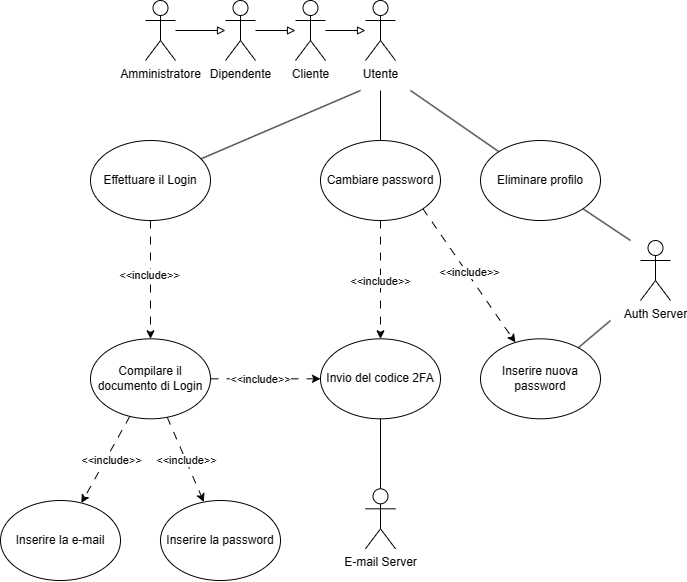
\includegraphics[width=1\textwidth]{images/UCD/RF1_login_UCD.png}
	Use Case Diagram (UCD) di RF1 "Login"
\end{figure}
Per descrivere questo use case, facciamo uso di due diagrammi delle attività swimlane:
\begin{figure}[H]
	\centering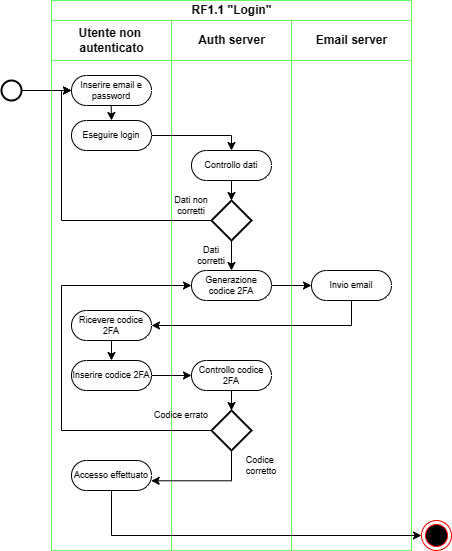
\includegraphics[width=1\textwidth]{images/Login_Swimlane.drawio.png}
	diagramma delle Attività swimlane del Login
\end{figure}
\begin{figure}[H]
	\centering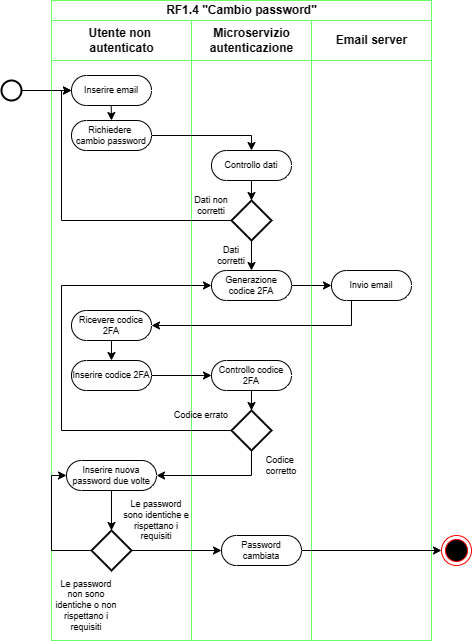
\includegraphics[width=1\textwidth]{images/password_change_swimlane.drawio.png}
	diagramma delle Attività swimlane del cambio password
\end{figure}
\subsection*{RF2 Registrazione}
\begin{figure}[H]
	\centering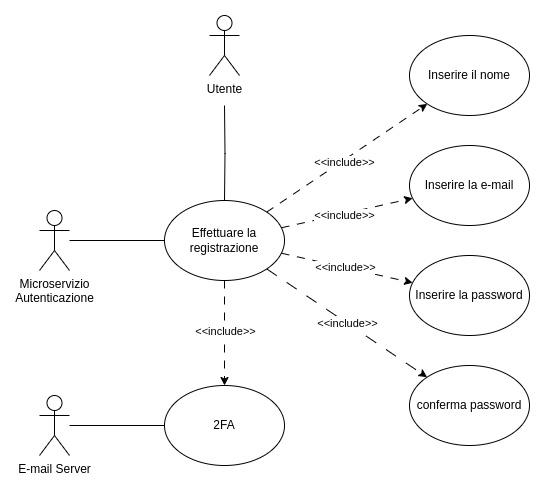
\includegraphics[width=1\textwidth]{images/UCD/RF2_registrazione_UCD.png}
	Use Case Diagram (UCD) di RF2 "Registrazione"
\end{figure}
Per descrivere questo use case, facciamo uso di un diagramma delle attività swimlane:
\begin{figure}[H]
	\centering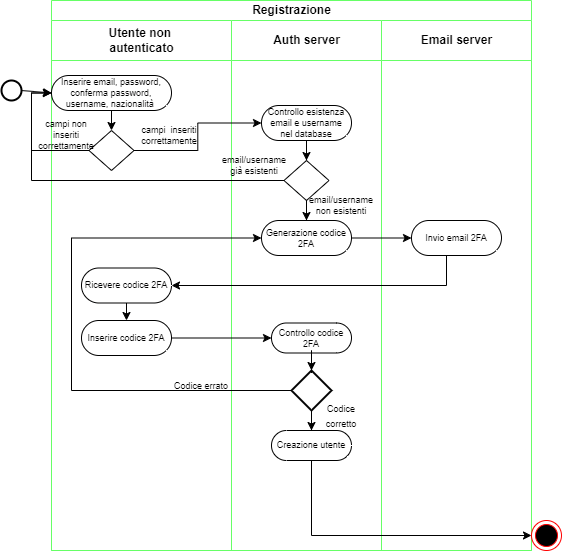
\includegraphics[width=1\textwidth]{images/Register_swimlane.drawio.png}
	diagramma delle Attività swimlane della registrazione
\end{figure}

\subsection*{RF4 Informazioni / Contatti}

\begin{figure}[H]
	\centering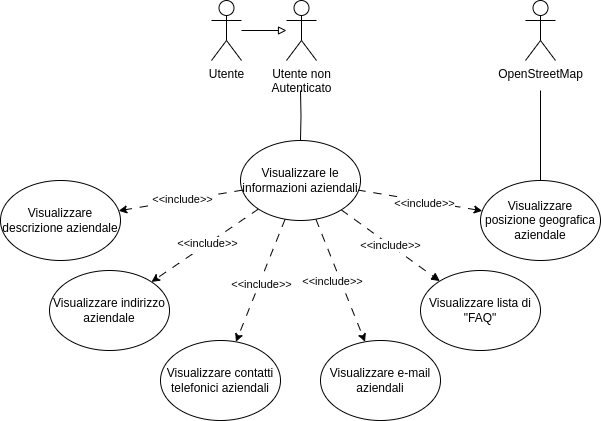
\includegraphics[width=1\textwidth]{images/UCD/RF4_infocontatti_UCD.png}
	Use Case Diagram (UCD) di RF4 "Informazioni / Contatti"
\end{figure}

\textbf{Titolo}: Informazioni / Contatti\\
\textbf{Descrizione}: L'utente cliccando la pagina "Informazioni / Contatti" visualizza le informazioni e i contatti dell'azienda, quali una descrizione, l'indirizzo e la posizione nella mappa, contatti telefonici, e-amil e FAQ.

\subsection*{RF3 Negozio Utente e RF5 Negozio Cliente}

\begin{figure}[H]
	\centering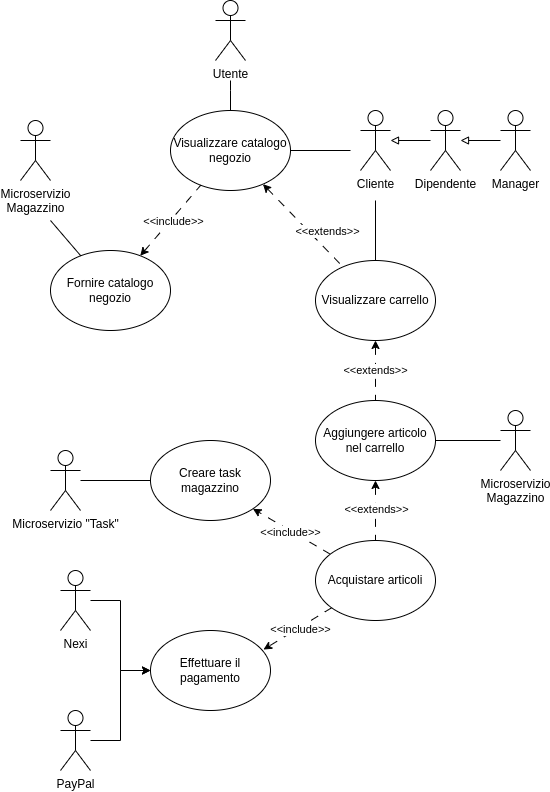
\includegraphics[width=1\textwidth]{images/UCD/RF3+5_negozio_UCD.png}
	Use Case Diagram (UCD) di RF3 e RF5 "Negozio"
\end{figure}

\begin{figure}[H]
	\centering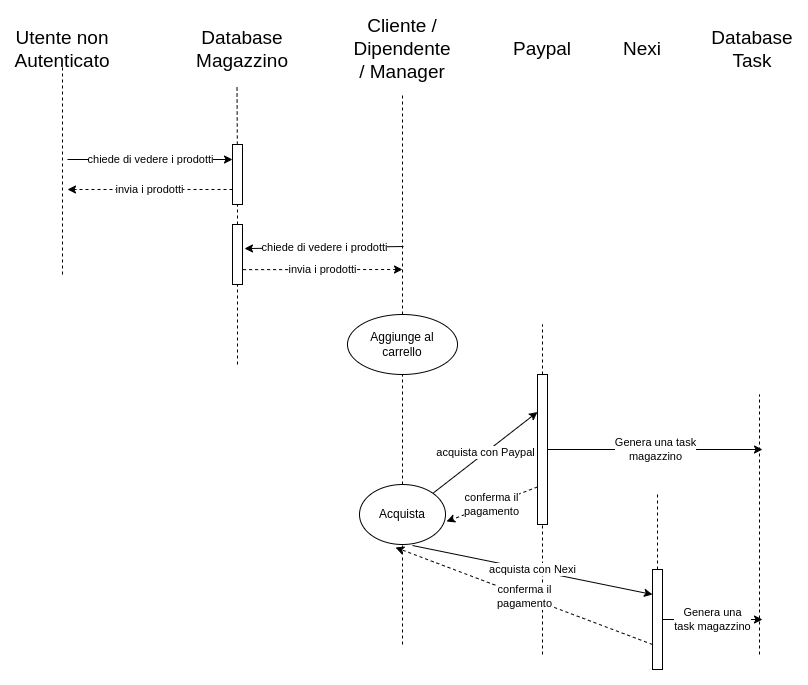
\includegraphics[width=1\textwidth]{images/negozio_sequence_diagram.png}
	diagramma delle Attività swimlane della registrazione
\end{figure}

\subsection*{RF6 Riparazione}
\begin{figure}[H]
	\centering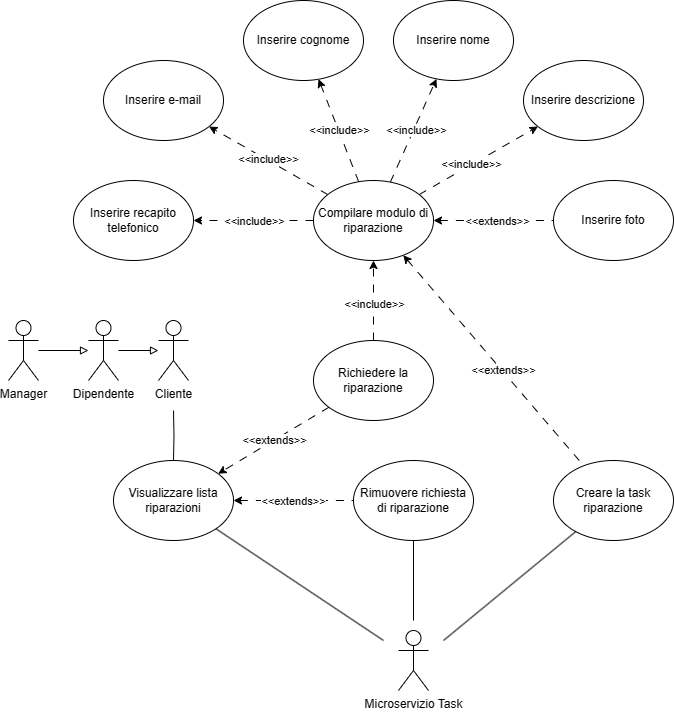
\includegraphics[width=1\textwidth]{images/UCD/RF6_riparazione_UCD.png}
	Use Case Diagram (UCD) di RF6 "Riparazione"
\end{figure}
\subsubsection*{Descrizione Use Case "Riparazione"}
\textbf{Titolo}: Riparazione \newline
\textbf{Riassunto}: Questo use case descrive come un utente può richiedere una riparazione e visualizzarne lo stato. \newline
\textbf{Descrizione}:
	\begin{enumerate}
		\item L'utente autenticato seleziona la pagina "Riparazioni";
		\item Il sito mostra lo stato delle riparazioni già richieste dall'utente [Exception 1];
		\item Il sito mostra un form per richiedere una nuova riparazione con i seguenti campi:
		\begin{itemize}
			\item nome[Exception 2];
			\item cognome[Exception 2]; 
			\item e-mail[Exception 2];
			\item numero di telefono[Exception 2];
			\item descrizione del problema[Exception 2];
			\item foto (( facoltativo ));
		\end{itemize}
		\item L'utente, appena compilato il form, può inviarlo premendo l'apposito pulsante;
		\item Il sistema, appena ricevuta la richiesta d.i riparazione, la inserisce nel sistema delle task come "task riparazione";
		
	\end{enumerate}
\textbf{Exceptions}
\begin{itemize}
	\item {[Exception 1]}: Se L'utente non ha nessuna riparazione richiesta, l'elenco sarà vuoto;
	\item {[Exception 2]}: Se l'utente non ha compilato i campi "nome","cognome","e-mail","numero di telefono","descrizione del problema" non può inviare la richiesta;
\end{itemize}
\subsection*{RF7 Assistenza}

\begin{figure}[H]
	\centering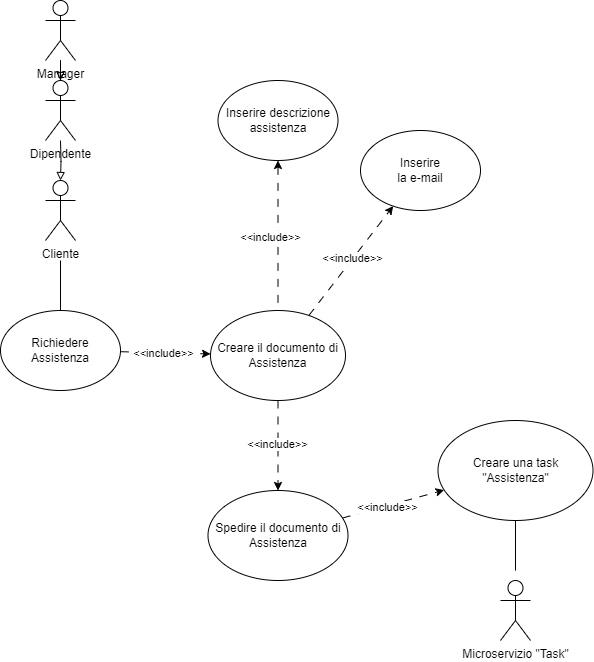
\includegraphics[width=1\textwidth]{images/UCD/RF7_assistenza_UCD.png}
	Use Case Diagram (UCD) di RF7 "Assistenza"
\end{figure}


\subsection*{RF8 Feedback}

\begin{figure}[H]
	\centering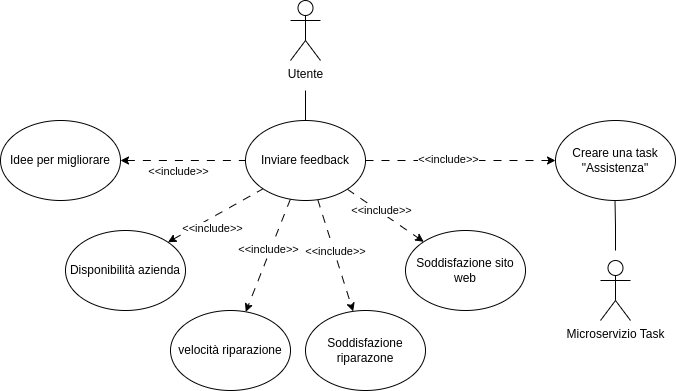
\includegraphics[width=1\textwidth]{images/UCD/RF8_feedback_UCD.png}
	Use Case Diagram (UCD) di RF8 "Feedback"
\end{figure}

\subsection*{RF9 Tasks}

\begin{figure}[H]
	\centering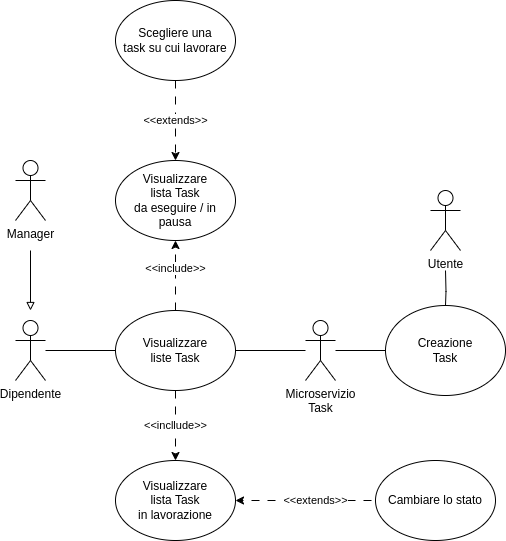
\includegraphics[width=1\textwidth]{images/UCD/RF9_task_UCD.png}
	Use Case Diagram (UCD) di RF9 "Task"
\end{figure}

Descrizione a parola qua

\begin{figure}[H]
	\centering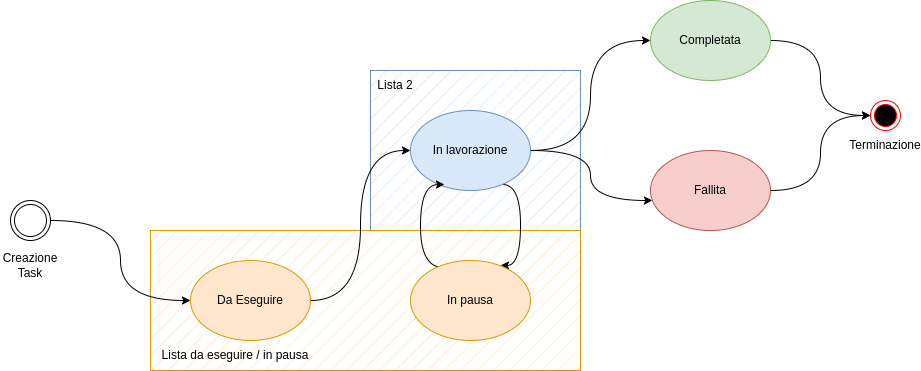
\includegraphics[width=1\textwidth]{images/state_diagram_task.png}
	State Diagram di RF9 "Task"
\end{figure}

\subsection*{RF10 Magazzino}
\begin{figure}[H]
	\centering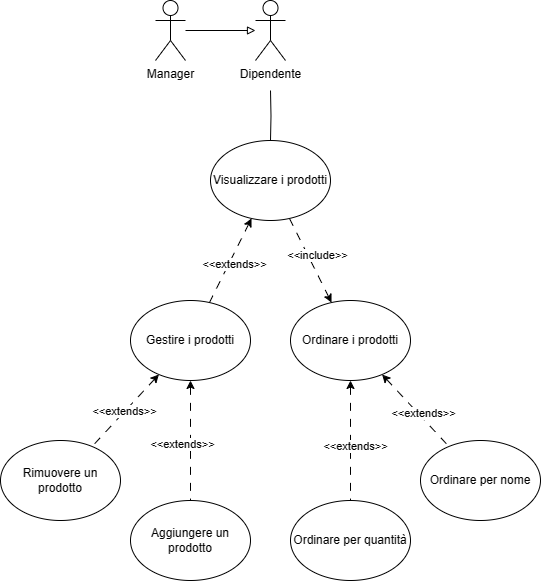
\includegraphics[width=1\textwidth]{images/UCD/RF10_magazzino_UCD.png}
	Use Case Diagram (UCD) di RF10 "Magazzino"
\end{figure}

\subsubsection*{Descrizione Use Case "Magazzino"}
\textbf{Titolo}: Magazzino \newline
\textbf{Riassunto}: Questo use case descrive come il manager ed i dipendenti possono visualizzare e gestire gli articoli presenti nel magazzino. \newline
\textbf{Descrizione}:
\begin{enumerate}
	\item Il dipendente seleziona la pagina "Magazzino";
	\item Il sito mostra la lista degli articoli disponibili [Exception 1];
	\item Il sito presenta un bottone in alto a destra etichettato "Ordina per" che permette di visualizzare gli articoli presenti per:
	\begin{itemize}
		\item nome[Exception 2];
		\item quantità[Exception 2];
	\end{itemize}
	\item Il sito presenta un bottone accanto ad ogni articolo etichettato "Rimuovi" che permette di eliminare quell'articolo dal magazzino;
	\item Il sito presenta un bottone in alto a destra etichettato "Aggiungi nuovo articolo" che permette di aggiungere un nuovo articolo.
	
\end{enumerate}
\textbf{Exceptions}
\begin{itemize}
	\item {[Exception 1]}: Se non vi sono articoli presenti nel sistema l'elenco sarà vuoto;
	\item {[Exception 2]}: Se il manager non ha compilato i campi "nome","cognome","data di nascita", "data di assunzione", "e-mail","password" non può creare il nuovo profilo dipendente;
	\item {[Exception 3]}: Se il dipendente non ha nessun work-tag assegnato la lista risulterà essere vuota;
\end{itemize}

\subsection*{RF11 Gestione Dipendenti}

\begin{figure}[H]
	\centering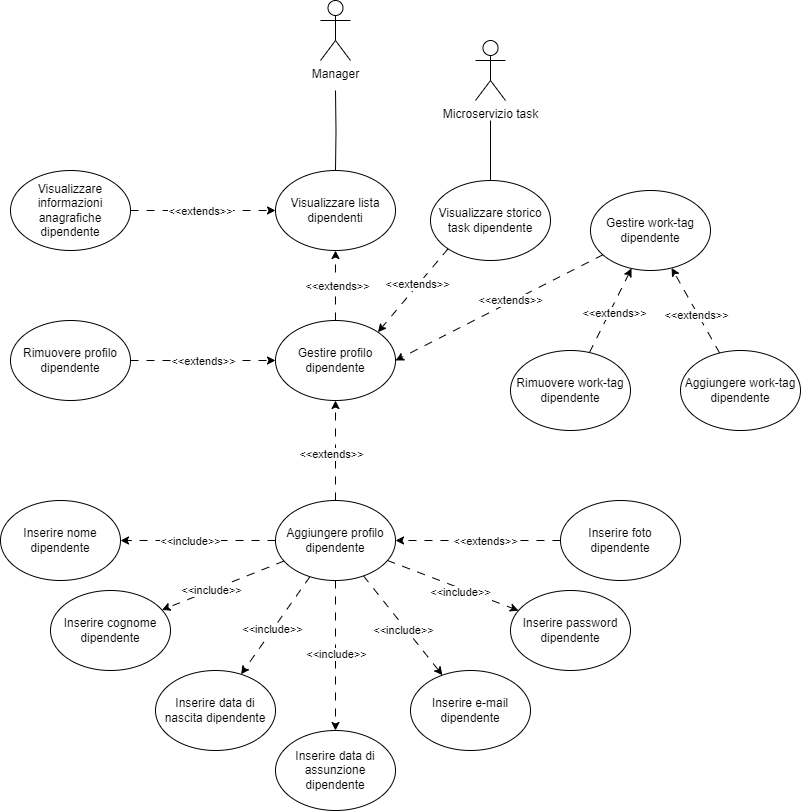
\includegraphics[width=1\textwidth]{images/UCD/RF11_gestionedipendenti_UCD.png}
	Use Case Diagram (UCD) di RF11 "Gestione Dipendenti
\end{figure}

\subsubsection*{Descrizione Use Case "Gestione Dipendenti"}
\textbf{Titolo}: Gestione Dipendenti \newline
\textbf{Riassunto}: Questo use case descrive come il manager può visualizzare e gestire i dipendenti. \newline
\textbf{Descrizione}:
\begin{enumerate}
	\item Il manager seleziona la pagina "Gestione Dipendenti";
	\item Il sito mostra la lista dei dipendenti [Exception 1];
	\item Il sito presenta un bottone in alto a destra etichettato "Aggiungi nuovo dipendente" che permette di creare un nuovo profilo inserendo i seguenti campi:
	\begin{itemize}
		\item nome[Exception 2];
		\item cognome[Exception 2]; 
		\item data di nascita[Exception 2];
		\item data di assunzione[Exception 2];
		\item e-mail[Exception 2];
		\item password[Exception 2];
		\item foto (( facoltativo ));
	\end{itemize}
	\item Il sito presenta un bottone accanto ad ogni dipendente etichettato "Rimuovi" che permette di eliminare quel profilo dipendente;
	\item Il sito presenta un bottone accanto ad ogni dipendente etichettato "Gestisci work-tag" che permette di visualizzare la lista di work-tag assegnati a quel dipendente [Exception 3], inoltre permette di:
	\begin{itemize}
		\item Aggiungere un nuovo work-tag;
		\item Rimuovere un work-tag;;
	\end{itemize}
	
\end{enumerate}
\textbf{Exceptions}
\begin{itemize}
	\item {[Exception 1]}: Se non vi sono dipendenti presenti nel sistema l'elenco sarà vuoto;
	\item {[Exception 2]}: Se il manager non ha compilato i campi "nome","cognome","data di nascita", "data di assunzione", "e-mail","password" non può creare il nuovo profilo dipendente;
	\item {[Exception 3]}: Se il dipendente non ha nessun work-tag assegnato la lista risulterà essere vuota;
\end{itemize}

\pagebreak

\section{Requisiti Non Funzionali}
Nel seguente capitolo vengono riportati i requisiti non funzionali (RNF) del sistema utilizzando tabelle strutturate e specificando misure facilmente misurabili.


\subsection*{RNF1 Intuitività e Accessibilità}
% table
\begin{center} % center the table
	\centering
	\begin{tabular}{ |p{3cm}|p{4cm}|p{4cm}|  }
		\hline
		\centering Proprietà & \qquad\quad Descrizione & \qquad\qquad Misura\\ % I found no other way...
		\hline
		Linguaggio Comprensibile & In media l’utente deve essere in grado di capire le funzionalità dell'applicazione con una
		sola lettura della descrizione. & In media, il numero di click errati che l'utente compie deve essere minore di 4. \\
		\hline
		Presenza della lingua Inglese e Italiana & Il sito presenta sia la lingua Italiana che quella Inglese, l'utente con un livello di lingua "A1" è in grado di leggere e comprendere il contenuto. & La scelta del vocabolario linguistico utilizzato è conforme con il vocabolario Italiano di livello A1 e Inglese livello A1.\\ % I found no other way...
		\hline
		Consistenza & Il sito deve avere un design consistente, utilizzando un singolo font e una palette fissa di colori. & numero di font utilizzati uguale a 1, numero di colori utilizzati minore di 6.  \\% I found no other way... 
		\hline
	\end{tabular}
\end{center}

\subsection*{RNF2 Sicurezza}
% table
\begin{center} % center the table
	\centering
	\begin{tabular}{ |p{3cm}|p{4cm}|p{4cm}|  }
		\hline
		\centering Proprietà & \qquad\quad Descrizione & \qquad\qquad Misura\\ % I found no other way...
		\hline
		Protezione dati & Il sito deve proteggere i dati sensibili utilizzando un algoritmo di hashing "SHA-3" per sarlvare e controllare le password e protocolli tls e https per ogni comunicazione tra utenti e servizi. & L'applicazione utilizza un algoritmo di hashing "SHA-3" nel salvataggio e controllo di password nel database e utilizza protocolli "tls" e "https" per ogni comunicazione tra utenti e servizi.\\
		\hline
		2 Factor Authentication (2FA) & Il sito deve verificare l'identità dell'utente attraverso il 2FA. & Impossibilità di accedere al sito senza 2FA.\\
		\hline
		Conformità password & La password di un utente deve avere una lunghezza minima di 10 caratteri e deve presentare almeno un numero,una lettera maiuscola, e un carattere speciale. &
		Numero dei caratteri maggiore di nove, presenza di almeno un numero,lettera maiuscola e carattere speciala dalla seguente lista:		\begin{verbatim} ! ? $ % ^ & * ( ) _ \end{verbatim} \begin{verbatim}- + = { [ } ] : ;\end{verbatim} \begin{verbatim}@ # | \ < , > . \end{verbatim} \\
		\hline
		
	\end{tabular}
\end{center}
\subsection*{RNF3 Privacy}
% table
\begin{center} % center the table
	\centering
	\begin{tabular}{ |p{3cm}|p{4cm}|p{4cm}|  }
		\hline
		\centering Proprietà & \qquad\quad Descrizione & \qquad\qquad Misura\\ % I found no other way...
		\hline
		GDPR & il sito deve essere conforme alle principali direttive del GDPR, tra cui il consenso esplicito per la raccolta dei dati, la trasparenza nell'uso dei dati, la possibilità di accesso e cancellazione dei dati personali da parte dell'individuo, e misure di sicurezza per proteggere tali dati. & Conforme al regolamento. \\
		\hline
	\end{tabular}
\end{center}
\subsection*{RNF4 Affidabilità e Disponibilità}
% table
\begin{center} % center the table
	\centering
	\begin{tabular}{ |p{3cm}|p{4cm}|p{4cm}|  }
		\hline
		\centering Proprietà & \qquad\quad Descrizione & \qquad\qquad Misura\\ % I found no other way...
		\hline
		Risultati desiderati & La probabilità che il sito fornisca i risultati desiderati senza interruzioni o tempi di inattività deve essere maggiore del 99\% (novantanove percento) & $\frac{\text{risultati ricevuti con successo}}{\text{risultati totali}}$ maggiore di 0.99 in media.\\ % There was no other way...
		\hline
		Operatività &  la probabilità che il sito rimanga operativo in un determinato momento
		indipendentemente dal numero di guasti già subiti dal sistema deve essere maggiore del 99\% (novantanove percento) & $ \frac{\text{secondi di attività dal lancio}}{\text{secondi totali dal lancio}}$ maggiore di 0.99 in media.\\
		\hline 
	\end{tabular}
\end{center}
\subsection*{RNF5 Performante}
% table
\begin{center} % center the table
	\centering
	\begin{tabular}{ |p{3cm}|p{4cm}|p{4cm}|  }
		\hline
		\centering Proprietà & \qquad\quad Descrizione & \qquad\qquad Misura\\ % I found no other way...
		\hline
		Aggiornamento negozio & Il sito deve elaborare l'inserimento di un articolo nel magazzino in meno di un secondo. & Il numero di secondi trascorsi da quanto viene premuto il bottone "inserisci articolo" a quando l'articolo è presente nel magazzino deve essere minore di uno. \\
		\hline 
		2 Factor Authentication (2FA)& Il sito deve inviare la mail di 2FA in meno di cinque secondi. & Secondi trascorsi da quando è stato richiesto l'invio di un coridce 2FA a quando il codice è presente nella mail minore di 5 (cinque) secondi. \\
		\hline
		Lista delle Task & Il sito deve aggiornare la lista delle task in meno di un secondo. & Il numero di secondi trascorsi per eseguire e terminare l'operazione di inserimento di una task nel database minore di 1. \\ 
		\hline

	\end{tabular}
\end{center}
\subsection*{RNF6 Compatibilità e Portabilità}
% table
\begin{center} % center the table
	\centering
	\begin{tabular}{ |p{3cm}|p{4cm}|p{4cm}|  }
		\hline
		\centering Proprietà & \qquad\quad Descrizione & \qquad\qquad Misura\\ % I found no other way...
		\hline
		Compatibilità dispositivi lato client & L'applicazione lato client  deve essere disponibile per dispositivi aventi un browser che supporta \begin{itemize}
		\item componenti html5 utilizzati
		\item https
		\item tls 1.2
		\end{itemize} &  L'applicazine ulizza https, tls 1,2 e html5.  \\
		\hline
		Compatibilità dispositivi lato server & L'applicazione lato server deve essere disponibile per computer che supportino: 
		\begin{itemize}
			\item Node js 18.18.0 LTS
		\end{itemize}
		&  L'applicazione utilizza Node js 18.18.0 LTS. \\
		\hline 
		Responsive su TV e monitor di PC e Laptop & Il sito deve potersi adattare alla dimensione degli schermi con Aspect Ratio da 4:3, 16:9, 21:9 & L'utente è in grado di eseguire correttamente ogni funzionalità dell'applicazione su schermi con aspectratio 4:3, 16:9 e 21:9. \\
		\hline
		Responsive su Smartphone & Il sito deve potersi adattare agli schermi dei seguenti Smartphone: 
		\begin{itemize}
			\item Iphone X,XR,11,\dots , 14
			\item Tutti i modelli Xiaomi dal 2018 in poi 
			\item Tutti i modelli Samsung dal 2018 in poi
			\item Tutti i modelli Motorola dal 2018 in poi 
			\item Tutti i modelli Huawei dal 2018 in poi 
		\end{itemize}
		&  L'utente è in grado di eseguire correttamente ogni funzionalità dell'applicazione sui dispositivi elencati. \\
		
		\hline
		
	\end{tabular}
\end{center}
\begin{center} % center the table
	\centering
	\begin{tabular}{ |p{3cm}|p{4cm}|p{4cm}|  }
		\hline
		Responsive su Tablet & Il sito deve potersi adattare agli schermi dei seguenti Tablet: 
		\begin{itemize}
			\item Ipad Air, Pro dal 2018 in poi
			\item Tutti i modelli Xiaomi dal 2018 in poi
			\item Tutti i modelli Samsung dal 2018 in poi
		\end{itemize} & L'utente è in grado di eseguire correttamente ogni funzionalità dell'applicazione sui dispositivi elencati. \\
		\hline
		
		
	\end{tabular}
\end{center}
\subsection*{RNF7 Mantenibilità e Scalabilità}
% table
\begin{center} % center the table
	\centering
	\begin{tabular}{ |p{3cm}|p{4cm}|p{4cm}|  }
		\hline
		\centering Proprietà & \qquad\quad Descrizione & \qquad\qquad Misura\\ % I found no other way...
		\hline
		Team di manutenzione &  Al sito deve essere affiancato, prima e dopo il rilascio ufficiale, un team di
		manutenzione che si occupi di testare ogni funzionalit`a periodicamente e
		che, su richiesta qualora ci siano problemi, sia pronto a intervenire tempestivamente
		 & E' presente un team che una volta al mese testa il sistema e le sue funzionalità, in grado di presentarsi all'azienda in meno di un giorno. \\
		\hline
		sito facilmente mantenibile & Il sito deve possedere le seguenti caratteristiche
		\begin{itemize}
			\item Il codice sorgente del back-end dev'essere modulare, utilizzando un'architetture a microserivizi
			\item Il codice sorgetne deve rispettare le linee guida del linguaggio scelto
		\end{itemize}
		& Conformità Linee guida Javascript, architettura divisa in microservizi.
		\\  \hline

	\end{tabular}
\end{center}
\subsection*{RNF8 Conformità}
\begin{center} % center the table
	\centering
	\begin{tabular}{ |p{3cm}|p{4cm}|p{4cm}|  }
		\hline
		\centering Proprietà & \qquad\quad Descrizione & \qquad\qquad Misura\\ % I found no other way...
		\hline
		Conformità leggi & L'applicazione deve essere conforme alle normative di legge in materia di siti web imposti dall'Unione Europea & Conforme ai regolamenti. \\
		\hline
		Conformità GDPR & L'applicazione deve essere conforme al GDPR, come descritto in RNF3 & Conforme ai regolamenti.\\
		\hline
		Conformità W3C WAI & L'applicazione deve essere conforme al W3C WAI (Web Accessibility Initiative) & Conforme ai regolamenti.\\ 
		\hline
	\end{tabular}

\end{center}


\chapter{Analisi del Contesto}

\section{Utenti e Sistemi Esterni}

Sono stati individuati tutti gli Utenti ed i Sistemi Esterni che fanno parte del funzionamento del sistema "Fix Mi".\\Segue una elencazione di ogni elemento con una descrizione breve adibita.


\subsection*{Utente non autenticato/Ospite}
Con il termine "Utente non autenticato" o "Ospite" si definisce una qualsiasi persona che abbia fatto accesso al sistema senza essersi identificati. L'Ospite è in grado di:
\begin{itemize}
	\item Accedere all'area "Negozio" per visualizzare il catalogo.
	\item Accedere all'area "Informazioni / Contatti" e visualizzarne i dettagli. 
	%tutti i dettagli in esso contenuti, tra cui numeri telefonici, indirizzi di posta elettronica e posizione geografica aziendale.
\end{itemize}


\subsection*{Cliente}

Con il termine "Cliente" si intende un Utente che abbia compiuto con successo la registrazione nel sistema e che successivamente abbia fatto l'accesso nel suo profilo. Il Cliente, oltre a potere accedere a tutti i servizi offerti ad un profilo "Utente", è in grado di
\begin{itemize}
	\item Inserire gli articoli dell'area "Negozio" nel proprio carrello e, successivamente, effettuarne l'acquisto.
	\item Accedere all'area "Riparazione" per visualizzare la lista di riparazioni in corso, creare una nuova richiesta di Riparazione o eliminarne una esistente.
	%\item Inviare feedback riguardo la qualità dei servizi offerti. (Lmao non ho ancora capito se questo c'è oppure no).
\end{itemize}
\subsection*{Dipendente}

Con il termine "Dipendente" si intende quella persona che abbia stipulato un contratto di lavoro con l'azienda. Il Dipendente, oltre a poter usufruire di tutti i servizi adibiti ad un profilo Cliente, può:
\begin{itemize}
	\item Accedere all'area "Magazzino" per visualizzare la lista dei prodotti posseduti, aggiungere un nuovo articolo o rimuoverne uno esistente.
	\item Accedere all'area "Task" per visualizzare la lista delle Task, crearne una nuova, contrassegnarla o rimuoverne una esistente. 
\end{itemize}

\subsection*{Manager}

Con il termine "Manager" si intende quella persona che abbia il completo controllo del sistema e dell'azienda. Il Manager, oltre a potere accedere a tutte le aree offerte al profilo Dipendente, è in grado di:
\begin{itemize}
	\item Accedere all'area "Gestione Dipendenti" per visualizzarne la lista, aggiungere un nuovo profilo Dipendente o eliminarne uno esistente.
\end{itemize}

\subsection*{Utente}
Con il termine "Utente" si intende qualsiasi persona che abbia un account, che sia di tipo "Cliente", "Dipendente", o "Manager"
\subsection*{Server Mail}
Attraverso la Server Mail, il sistema è in grado di mandare e ricevere e-mail. 

\subsection*{Database}
Il database memorizza il catalogo del negozio, l'inventario del magazzino e le informazioni riguardanti i profili gestiti dal sistema (es. e-mail e password).

\subsection*{PayPal e Nexi}
I servizi esterni "PayPal" e "Nexi" permettono al Cliente di effettuare acquisti all'interno del sistema.

\subsection*{OpenStreetMap}
Il servizio esterno "OpenStreetMap" fornisce dati geografici al sistema.%per visualizzare la posizione aziendale geografica in cartina.

\subsection*{Microservizio Autenticazione}
Con il termine "Microservizio Autenticazione" si intende il microservizio dell'applicazione che si occupa di gestire l'autenticazione degli utenti e il processo di login,registrazione e cambio password
\subsection*{Microservizio Task}
Con il termine "Microservizio Task" si intende il microservizio dell'applicazione che si occupa della gestione delle task.
\subsection*{Email Server}
Con il termine "Email Server" si intende il server aziendale per la gestione delle Email.
\begin{itemize}
	\item permette l'invio dei codici 2FA ("2 Factor Authentication")
	\item contiene le Email aziendali dei dipendenti e del manager
	\item viene usato dai dipendenti e dal manager per l'invio di email 
\end{itemize}
\subsection*{Microservizio Magazzino}
Con il termine "Microservizio Magazzino" si intende il microservizio dell'applicazione che si occupa di gestire l'inventario aziendale.


\section{Diagramma di Contesto}

Il seguente diagramma di contesto rappresenta l'applicazione "Fix Mi" da un punto di vista generale e riassuntivo.

\begin{figure}[H]
	\centering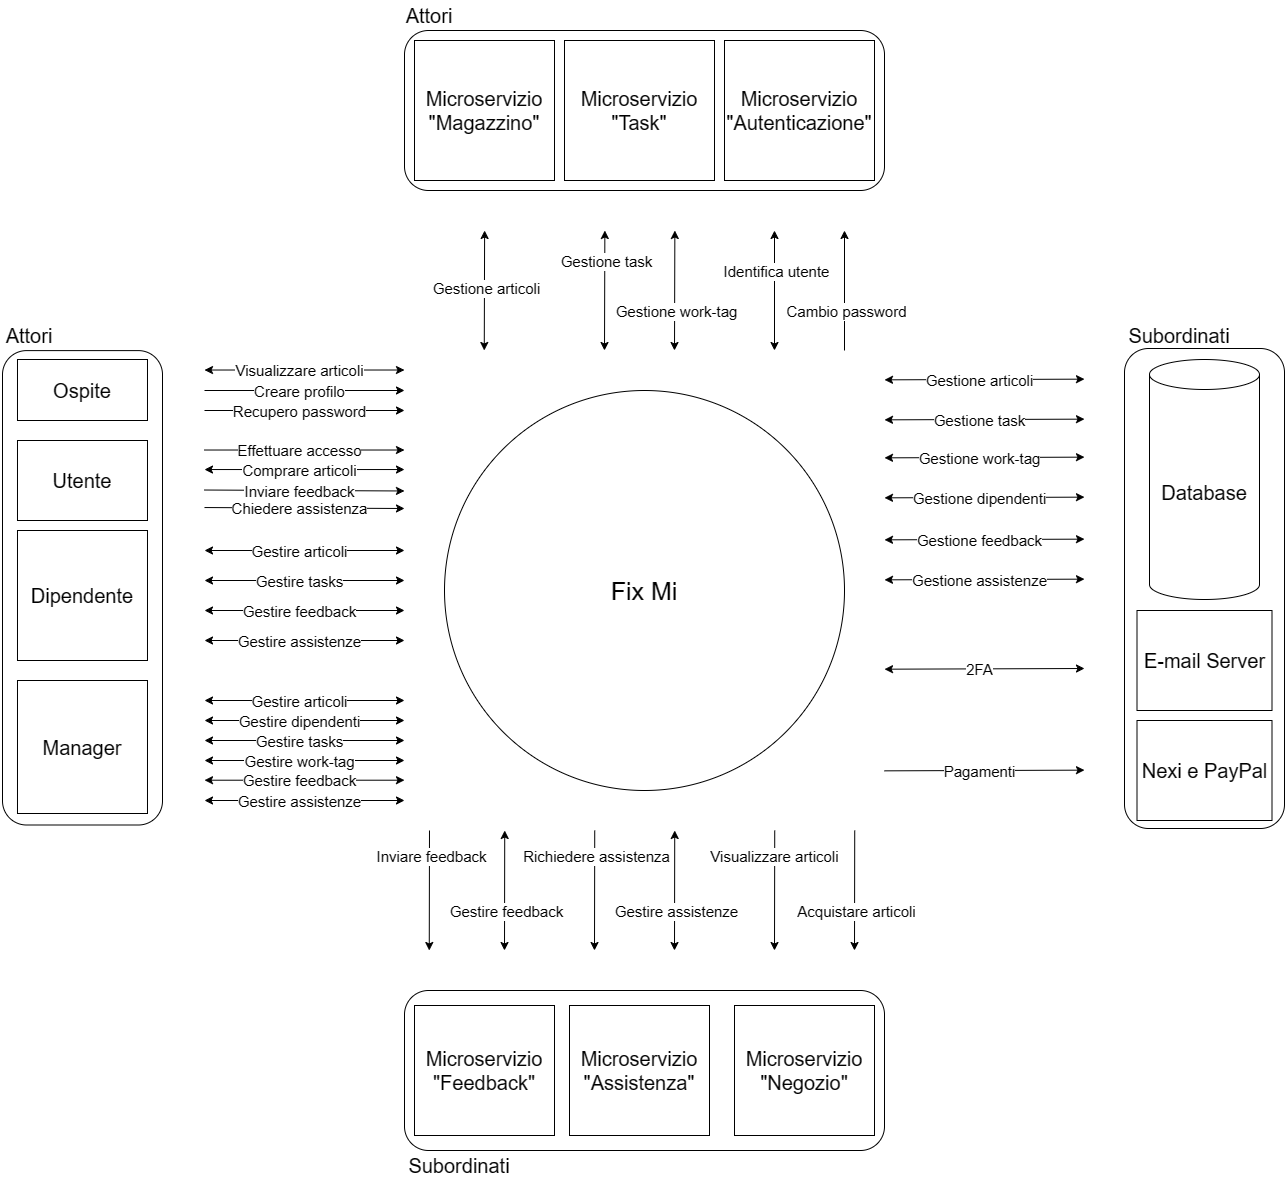
\includegraphics[width=1\textwidth]{images/Diagrammi_Contesto/Diagramma_Contesto_FixMi.png}
	Diagramma di contesto dell'applicazione "Fix Mi".
\end{figure}

I seguenti diagrammi di contesto rappresentano tutti i microservizi che, nell'insieme, compongono "Fix Mi".

\begin{figure}[H]
	\centering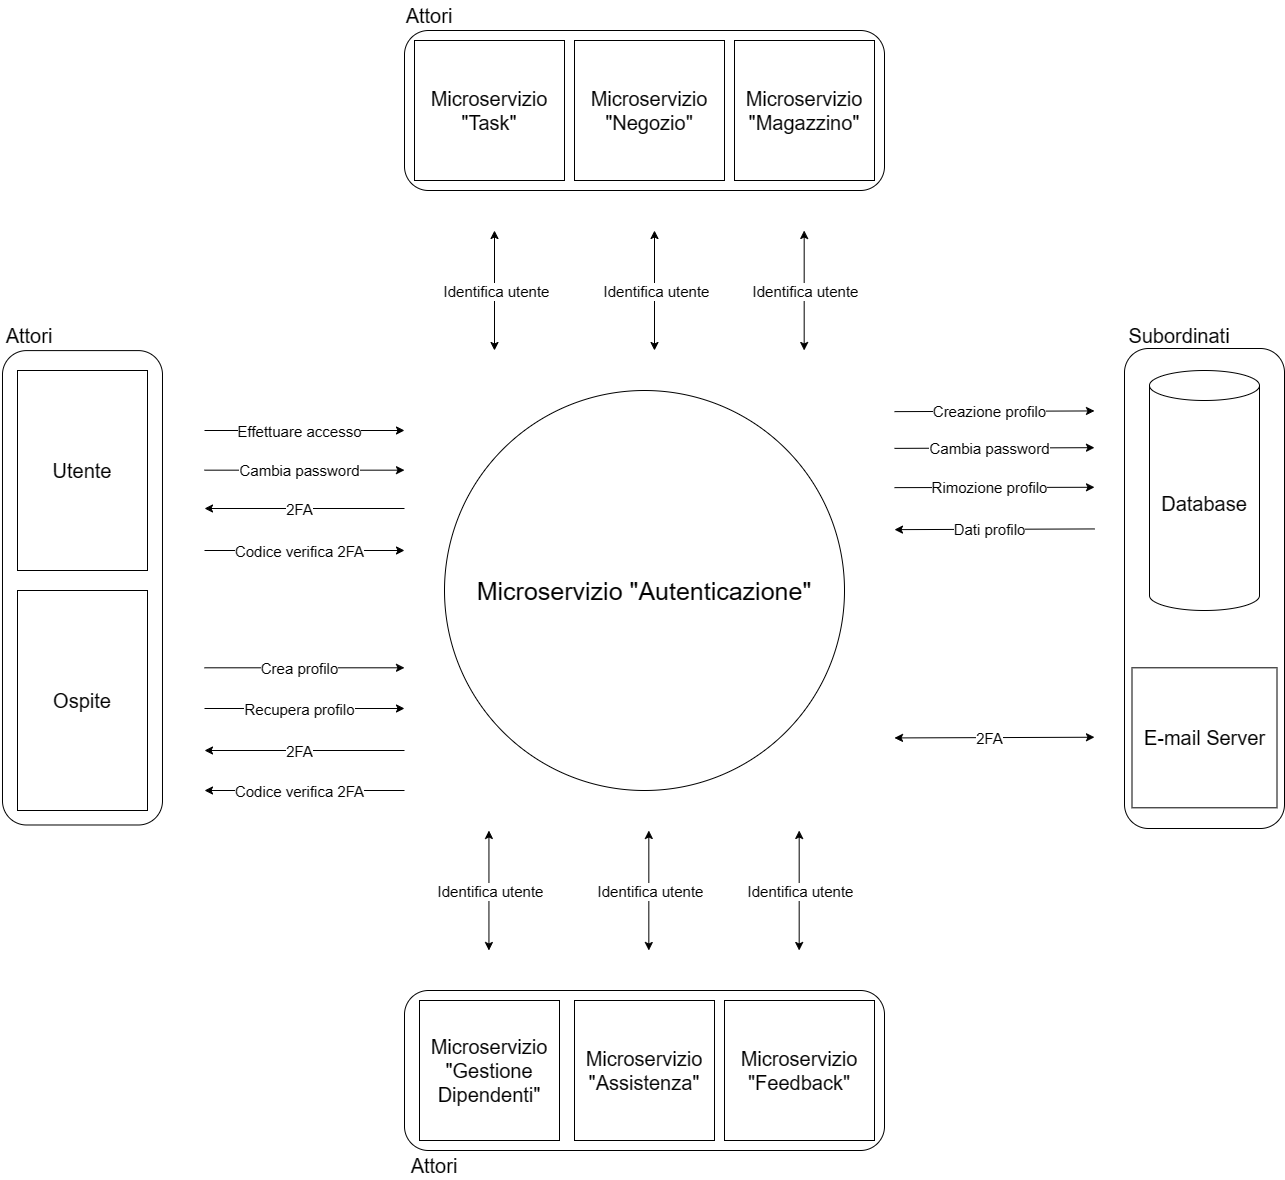
\includegraphics[width=1\textwidth]{images/Diagrammi_Contesto/Diagramma_Contesto_Autenticazione.png}
	Diagramma di contesto del microservizio "Autenticazione".
\end{figure}

\begin{figure}[H]
	\centering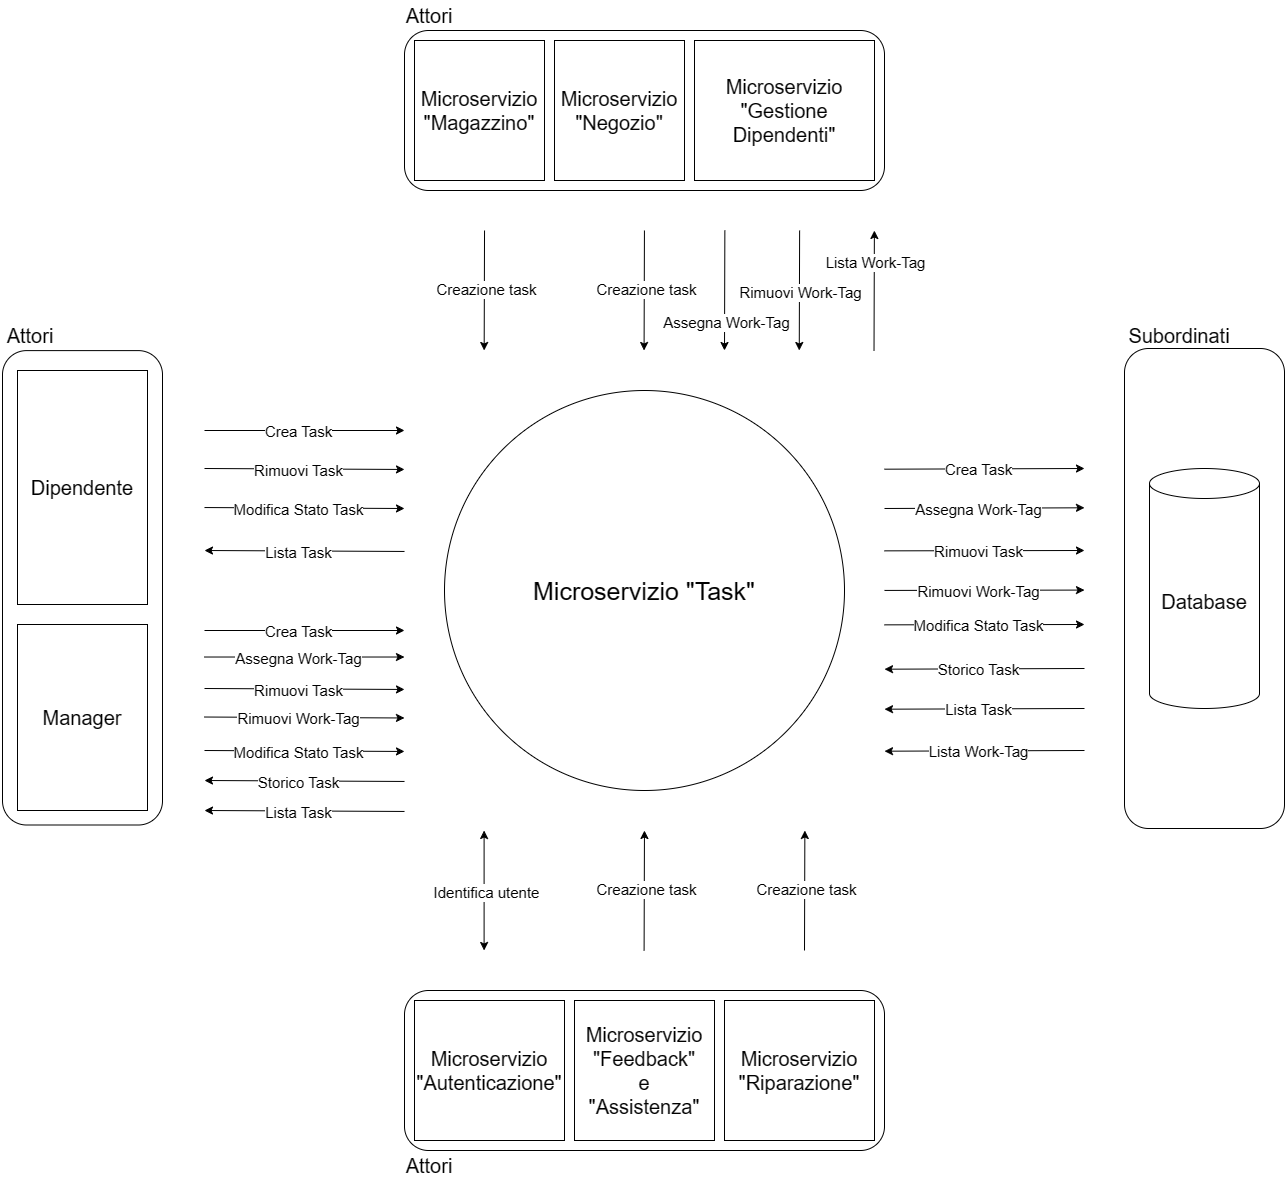
\includegraphics[width=1\textwidth]{images/Diagrammi_Contesto/Diagramma_Contesto_Task.png}
	Diagramma di contesto del microservizio "Task".
\end{figure}

\begin{figure}[H]
	\centering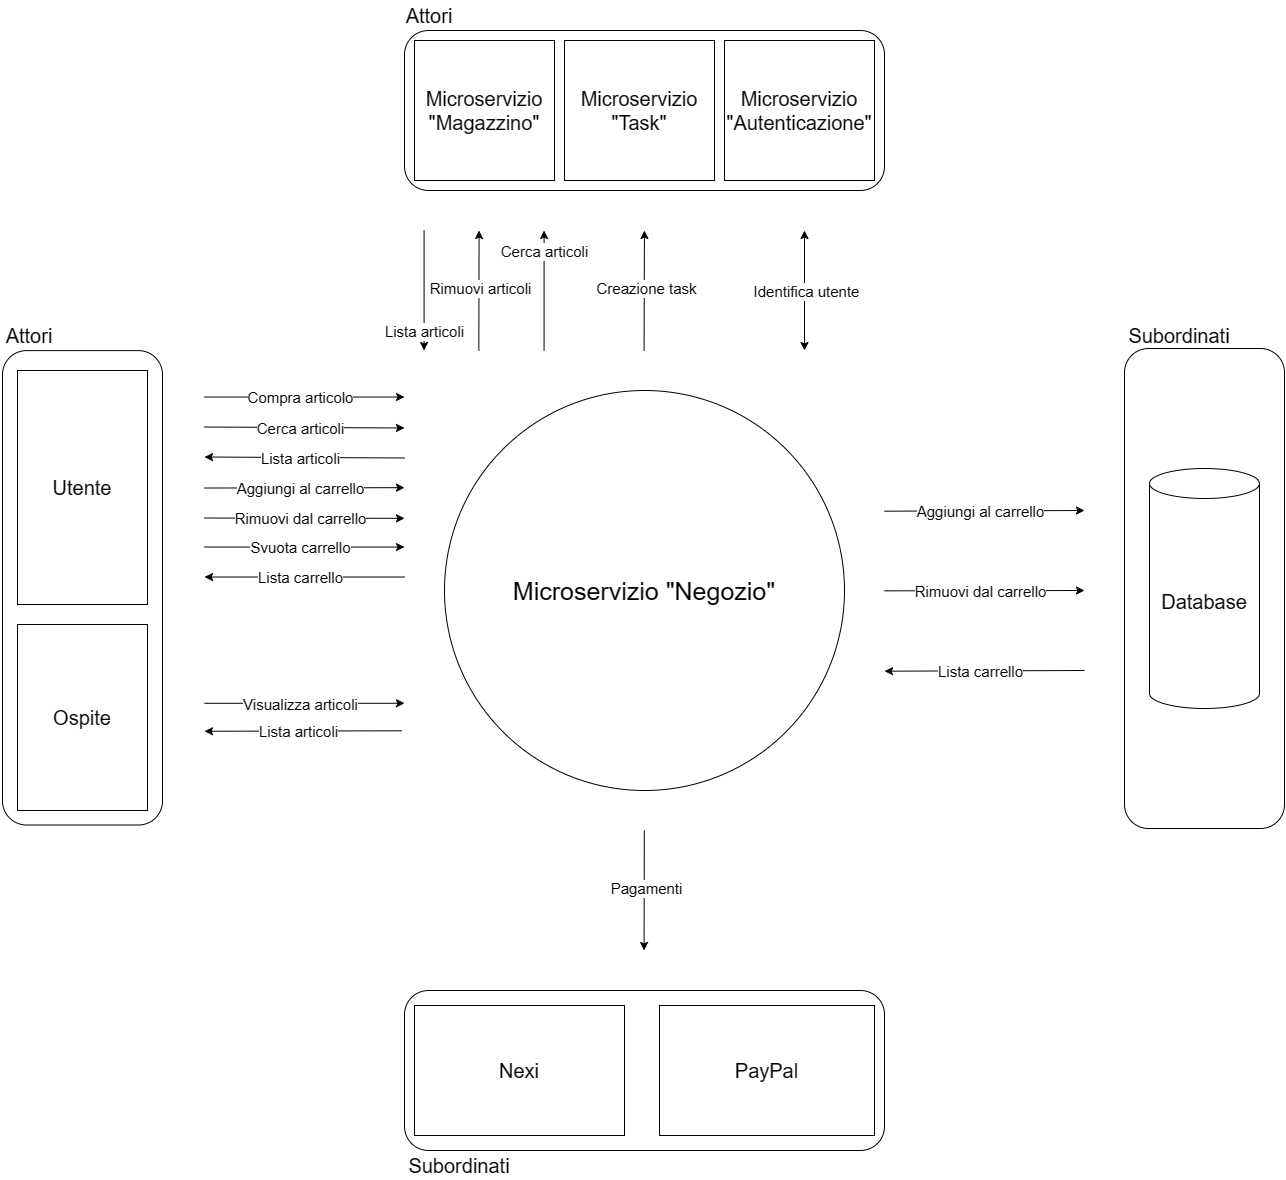
\includegraphics[width=1\textwidth]{images/Diagrammi_Contesto/Diagramma_Contesto_Negozio.png}
	Diagramma di contesto del microservizio "Negozio".
\end{figure}

\begin{figure}[H]
	\centering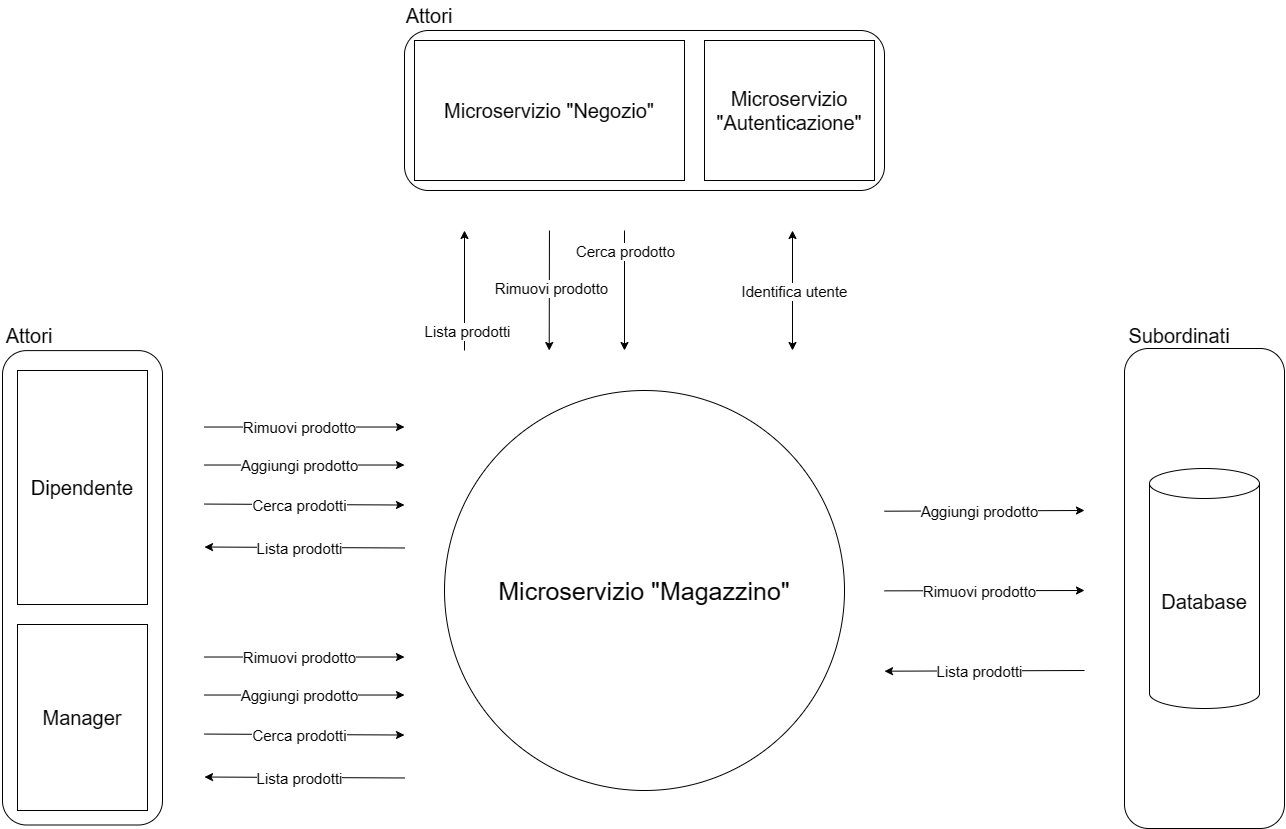
\includegraphics[width=1\textwidth]{images/Diagrammi_Contesto/Diagramma_Contesto_Magazzino.png}
	Diagramma di contesto del microservizio "Magazzino".
\end{figure}
\begin{figure}[H]
	\centering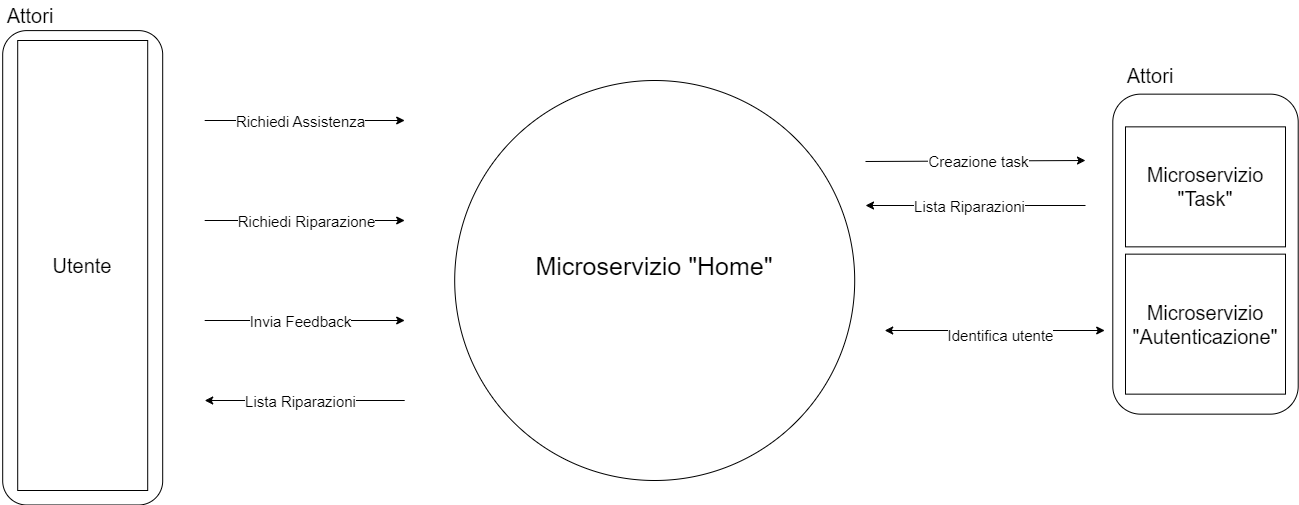
\includegraphics[width=1\textwidth]{images/Diagrammi_Contesto/Diagramma_Contesto_Home.png}
	Diagramma di contesto del microservizio "Home"
\end{figure}

\begin{figure}[H]
	\centering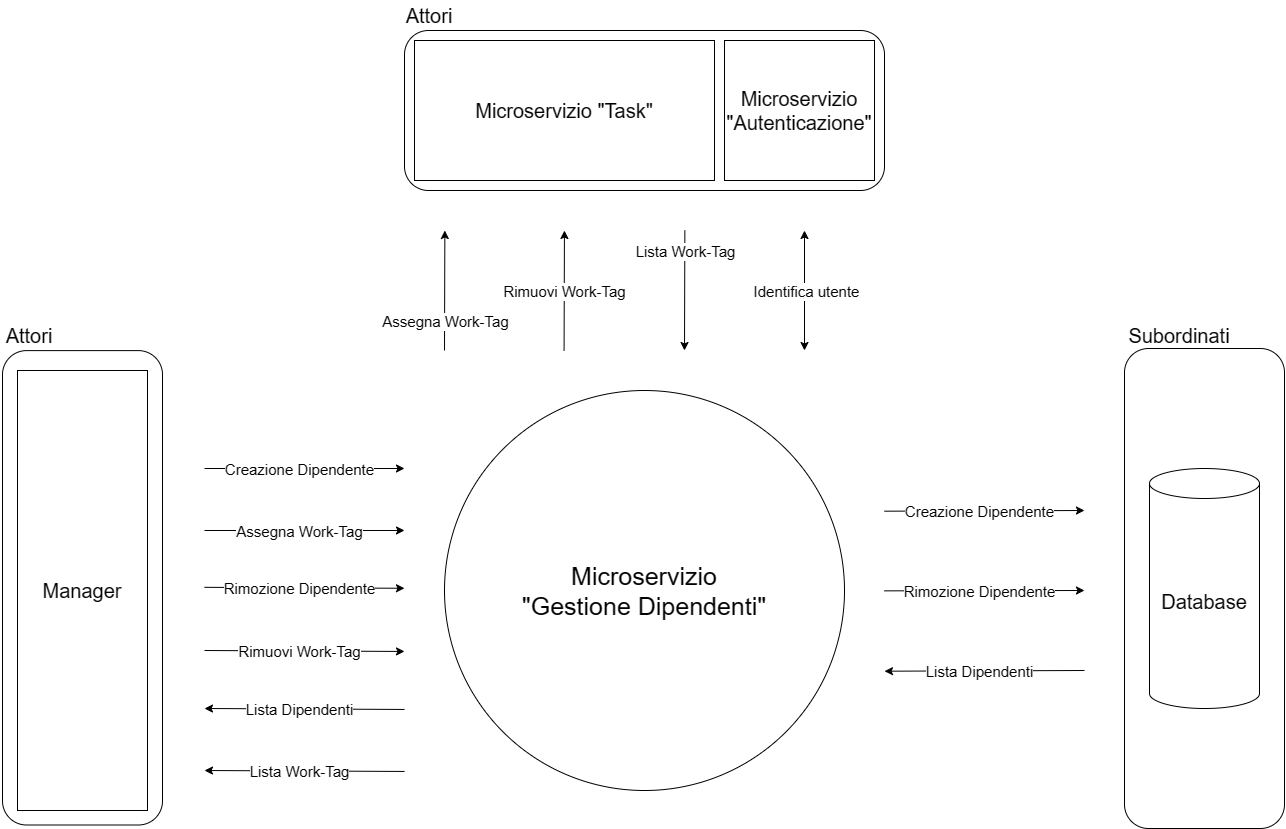
\includegraphics[width=1\textwidth]{images/Diagrammi_Contesto/Diagramma_Contesto_Dipendenti.png}
	Diagramma di contesto del microservizio "Gestione Dipendenti".
\end{figure}

\chapter{Analisi dei Componenti}
Nel presente capitolo viene presentata l’architettura in termini di componenti interni al sistema definiti sulla base dei requisiti analizzati nei precedenti documenti, minimizzando il livello di coesione. Viene poi adottato l’uso di Component Diagram per rappresentare l’interconnessione tra i vari componenti, identificando quindi le interfacce tra questi e verso sistemi esterni. Viene infine valutato il livello di accoppiamento tra i componenti.


\section{Definizione dei Componenti}
In questa sezione vengono definiti i componenti.

\subsection*{Autenticazione}
\uline{\textit{Descrizione}}: 
Sono stati considerati i requisiti funzionali \textbf{RF1}, \textbf{RF2} e la definizione del microservizio "Autenticazione" nel documento "Analisi dei requisiti"
Capitolo 3.2.3 "Design del Back End - Descrizione Microservizi".\\
È stata quindi definita la componente "Autenticazione", che gestirà tutte le operazioni relative all'autenticazione degli utenti.\\
Questa componente, infatti, sarà centrale al funzionamento del microservizio autenticazione, da cui prende il nome.\\
La componente si interfaccerà  con il database per la modifica, lettura, creazione ed eliminazione dei dati di autenticazione degli utenti dell'applicazione.\\
La componente si interfaccerà con le componenti "Login", "Registrazione" e "Cambio password", anche esse parte del microservizio autenticazione, per permetterne la funzionalità.\\
\subsubsection*{Sistema Token Utente}
La componente, per permettere all'utente di mantenere la propria sessione dopo il login, utilizzerà un sistema di "token utente".
Il token utente è un oggetto, generato dalla componente in fase di accesso, che identifica univocamente un utente e il suo ruolo(cliente, dipendente o manager).\\
A questo scopo, la componente fornirà il token alla componente "Login" e "Registrazione" su richiesta.\\
Ogni componente che, per diverse funzionalità, dovrà interagire con un utente autenticato  e verificare che abbia un ruolo sufficiente dovrà prima richiedere il proprio token all'utente, 
e successivamente inviarlo a questa componente per la verifica.

\subsection*{Login}
\uline{\textit{Descrizione}}:
È stato considerato il requisito funzionale \textbf{RF1}.\\
È stata quindi definita la componente "Login", che gestirà l'operazione di accesso da parte di un utente dell'applicazione, utilizzando le proprie credenziali.\\
La componente si appoggerà alla componente "Autenticazione" per la verifica delle credenziali fornite dall'utente.\\ 
La componente si interfaccerà con il Server Mail per l'invio del codice 2 Factor Authentication alla E-mail dell'utente, in modo da completare il login.\\
A login completato, la componente si interfaccerà con la componente "Autenticazione" per ottenere il token utente, e lo fornirà all'utente stesso.

\subsection*{Cambio Password}
\uline{\textit{Descrizione}}:
È stato considerato il requisito funzionale \textbf{RF1}.\\
È stata quindi definita la componente "Cambio Password", che gestirà l'operazione di cambio/recupero password richiesta da un utente.
La componente richiederà all'utente di inserire la propria E-mail.\\
La componente si appoggerà alla componente "Autenticazione" per verificare se la mail fornita dall'utente è associata a un utente già esistente, e per aggiornare la password a operazione completata.\\
La componente si interfaccerà con il Server Mail per l'invio del codice 2 Factor Authentication alla E-mail dell'utente, in modo da completare l'operazione

\subsection*{Registrazione}
\uline{\textit{Descrizione}}:
È stato considerato il requisito funzionale \textbf{RF2}.\\
È stata quindi definita la componente "Registrazione", che gestirà l'operazione di registrazione richiesta da un ospite.\\
La componente richiederà all'ospite di inviare i dati necessari per la registrazione, ossia nome/username, email e password.\\
La componente si appoggerà alla componente "Autenticazione" per verificare che la mail fornita dall'utente non sia già associata a un determinato account, e per richiedere la creazione del nuovo account a operazione completata.\\
La componente si interfaccerà con il Server Mail per l'invio del codice 2 Factor Authentication alla E-mail dell'ospite, in modo da poter completare la registrazione.\\
A registrazione completata ,la componente si interfaccerà con la componente "Autenticazione" per ottenere il token utente, e lo fornirà all'utente stesso.

\subsection*{Negozio}
\uline{\textit{Descrizione}}:
Sono stati considerati i requisiti funzionali\textbf{RF3} e \textbf{RF5}.\\
È stata quindi definita la componente "Negozio", che gestirà le funzionalità accessibili dall'utente attraverso la pagina con lo stesso nome.\\
La componente, per verificare l'identità dell'utente, richiederà allo stesso il proprio token utente, per poi verificarlo inviandolo alla componente "Autenticazione".\\
La componente, su richiesta dell'utente, fornirà la lista degli articoli acquistabili nel negozio, mostrando per ogni articolo nome, foto e descrizione. Per fare ciò, la componente dovrà comunicare con la componente "Magazzino".\\
Inoltre l'utente potrà cercare determinati articoli specificando una stringa che deve essere contenuta nella descrizione.\\
La componente, su richiesta dell'utente, aggiungerà l'articolo scelto al carrello dello stesso. Per fare ciò, la componente dovrà comunicare con la componente "Carrello", descritta di seguito. 
\subsection*{Carrello}
\uline{\textit{Descrizione}}:
È stato considerato il requisito funzionale \textbf{RF5}.\\
È stata quindi definita la componente "Carrello", che gestirà il carrello degli utenti e che permetterà l'acquisto degli articoli presenti nello stesso.\\
La componente, per verificare l'identità dell'utente, richiederà allo stesso il proprio token utente, per poi verificarlo inviandolo alla componente "Autenticazione".\\
\subsubsection*{Gestione Carrello}
La componente, su richiesta dell'utente, fornirà la lista degli articoli presenti nel proprio carrello.\\
La componente, su richiesta dell'utente, rimuoverà dal proprio carrello un determinato articolo o tutti gli articoli.\\
La componente, su richiesta della componente "Negozio", aggiungerà un determinato articolo al carrello dell'utente.\\
Per svolgere le operazioni descritte in questa sezione, la componente dovrà interfacciarsi con il database.
\subsubsection*{Acquisto}
La componente permetterà all'utente di acquistare gli articoli presenti nel proprio carrello.\\
Per fare ciò, la componente si interfaccerà con i sistemi di pagamento esterni "Nexi" e "Paypal".\\
A pagamento completato, la componente richiederà alla componente "Task" la creazione di una task "Magazzino". 
Questa servirà ai dipendenti per poter prendere dal magazzino gli articoli acquistati. 

\subsection*{Riparazione}
\uline{\textit{Descrizione}}:
È stato considerato il requisito funzionale \textbf{RF6}.\\
È stata quindi definita la componente "Riparazione", che gestirà il processo di "Richiesta Riparazione" da parte di un utente.\\
La componente, per verificare l'identità dell'utente, richiederà allo stesso il proprio token utente, per poi verificarlo inviandolo alla componente "Autenticazione".\\
La componente richiederà all'utente i dati della riparazione che desidera chiedere, ossia:
\begin{itemize}
	\item telefono
	\item email
	\item cognome
	\item nome
	\item descrizione
	\item foto(opzionale)
\end{itemize}
Una volta inviata la richiesta di riparazione, la componente richiederà alla componente "Task" la creazione di una task "Riparazione" con i dettagli forniti dall'utente, 
in modo che possa essere presa in carico da un dipendente.\\
La componente, su richiesta, fornisce all'utente la lista delle riparazioni che ha richiesto in precedenza, e il loro stato.

\subsection*{Assistenza}
\uline{\textit{Descrizione}}:
È stato considerato il requisito funzionale \textbf{RF7}.\\
È stata quindi definita la componente "Assistenza", che gestirà il processo di "Richiesta Assistenza".\\
La componente, per verificare l'identità dell'utente, richiederà allo stesso il proprio token utente, per poi verificarlo inviandolo alla componente "Autenticazione".\\
La componente richiederà all'utente i dati riguardanti la propria richiesta di riparazione, ossia:
\begin{itemize}
	\item descrizione
	\item E-mail
\end{itemize}
Una volta inviata la richiesta di assistenza, la componente richiederà alla componente "Task" la creazione di una task "Assistenza",
in modo che possa esssere presa in carico da un dipendente.

\subsection*{Feedback}
\uline{\textit{Descrizione}}:
È stato considerato il requisito funzionale \textbf{RF8}.\\
È stata quindi definita la componente "Feedback", che gestirà il processo di "Invio Feedback".\\
La componente, per verificare l'identità dell'utente, richiederà allo stesso il proprio token utente, per poi verificarlo inviandolo alla componente "Autenticazione".\\
La componente richiederà all'utente i dati riguardanti il feedback che desidera inviare, ossia:
\begin{itemize}
	\item disponibilità azienda
	\item velocità riparazione
	\item soddisfazione riparazione
	\item soddisfazione sito web
	\item idee per migliorare
\end{itemize}
Una volta inviato il feedback, la componente richiederà alla componente "Task" la creazione di una task "Assistenza",
in modo che possa esssere presa in carico da un dipendente.

\subsection*{Task}
\uline{\textit{Descrizione}}:
È stato considerato il requisito funzionale \textbf{RF9}.\\
È stata quindi definita la componente "Task", che si occupa della gestione del sistema Task dell'applicazione.\\
La componente, per verificare l'identità dell'utente e il suo ruolo(dipendente o manager), richiederà allo stesso il proprio token utente, per poi verificarlo inviandolo alla componente "Autenticazione".\\

\subsubsection*{Dipendente/Manager}
La componente permette al dipendente di vedere la lista delle task che può svolgere in base alle proprie "work-tag".\\
La componente permette al dipendente di assegnarsi una task da svolgere, e vedere le task su cui sta lavorando.\\
La componente permette al dipendente di cambiare lo stato di una determinata task su cui sta lavorando.
\subsubsection*{Altre Componenti}
La componente permette alle altre componenti di leggere la lista delle task e di crearne nuove.\\\\
Per permettere tutte le operazioni di lettura e creazione task, la componente si deve interfacciare al database.


\subsection*{Magazzino}
\uline{\textit{Descrizione}}:
È stato considerato il requisito funzionale \textbf{RF10}.\\
È stata quindi definita la componente "Magazzino", che si occupa della gestione, lettura, creazione ed eliminazione degli articoli presenti dentro al magazzino dell'azienda.\\
La componente, per verificare l'identità dell'utente e il suo ruolo(dipendente o manager), richiederà allo stesso il proprio token utente, per poi verificarlo inviandolo alla componente "Autenticazione".\\
La componente permette ai dipendenti e al manager di visualizzare gli articoli presenti nel magazzino, aggiungerne di nuovi e rimuovere quelli già presenti. Per fare ciò, la componente si interfaccia con il database.
La componente permette alla componente "Negozio" di prendere la lista degli articoli disponibili. 


\subsection*{Gestione Dipendenti}
\uline{\textit{Descrizione}}:
È stato considerato il requisito funzionale \textbf{RF11}\\
È stata quindi definita la componente "Gestione Dipendenti", che permette al manager la visualizzazione, aggiunta, modifica e rimoazione dei profili dei dipendenti dell'azienda.\\
La componente, per verificare l'identità dell'utente e il suo ruolo(manager), richiederà allo stesso il proprio token utente, per poi verificarlo inviandolo alla componente "Autenticazione".\\
La componente permette al manager di visualizzare la lista dei propri dipendenti, e le informazioni anagrafiche di ognuno.\\
La componente permette al manager di visualizzare lo storico delle task svolte da un determinato dipendente, interfacciandosi con la componente "Task".\\
La componente permette al manager di gestire le work-tag di un determinato dipendente, potendo aggiungerne di nuove o rimuovere quelle già esistenti.\\
La componente permette al manager di rimuovere il profilo di un dipendente.\\
La componente permette al manager di aggiungere un nuovo profilo dipendente, specificando:
\begin{itemize}
	\item nome
	\item cognome
	\item data di nascita
	\item data di assunzione
	\item E-mail
	\item password
	\item foto(opzionale)
\end{itemize}
Per la creazione del profilo, la componente si interfaccia con il database e, per salvare i dati di autenticazione, con la componente "Autenticazione".

\section{Diagramma dei Componenti}

Per semplificare i collegamenti a livello grafico abbiamo diviso in due grafici diversi le componenti che riguardano l'autenticazione dal il resto delle componenti.

\begin{figure}[H]
	\centering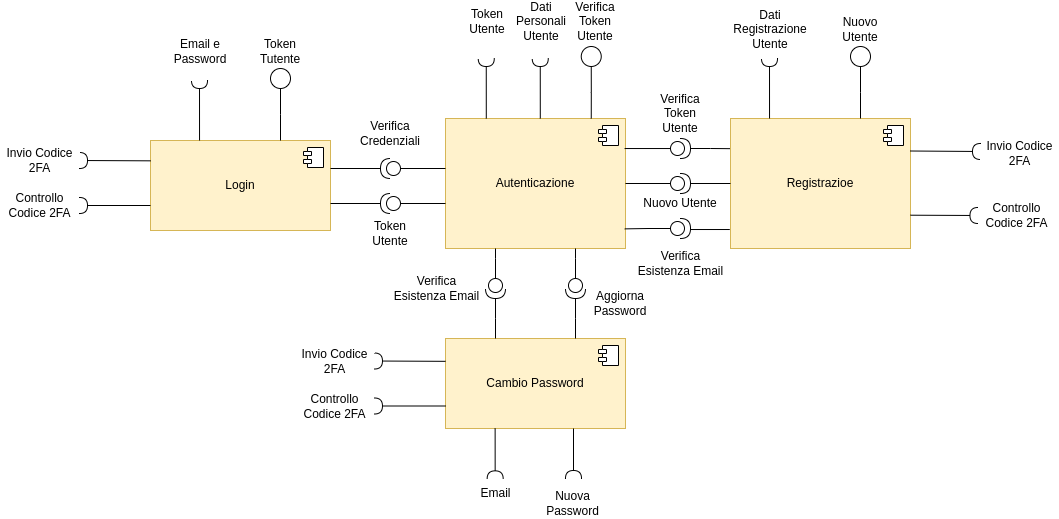
\includegraphics[width=1\textwidth]{images/autenticazione_diagramma_dei_componenti.png}
	Diagramma delle Componenti 1 per l'applicazione FixMi
\end{figure}

\begin{figure}[H]
	\centering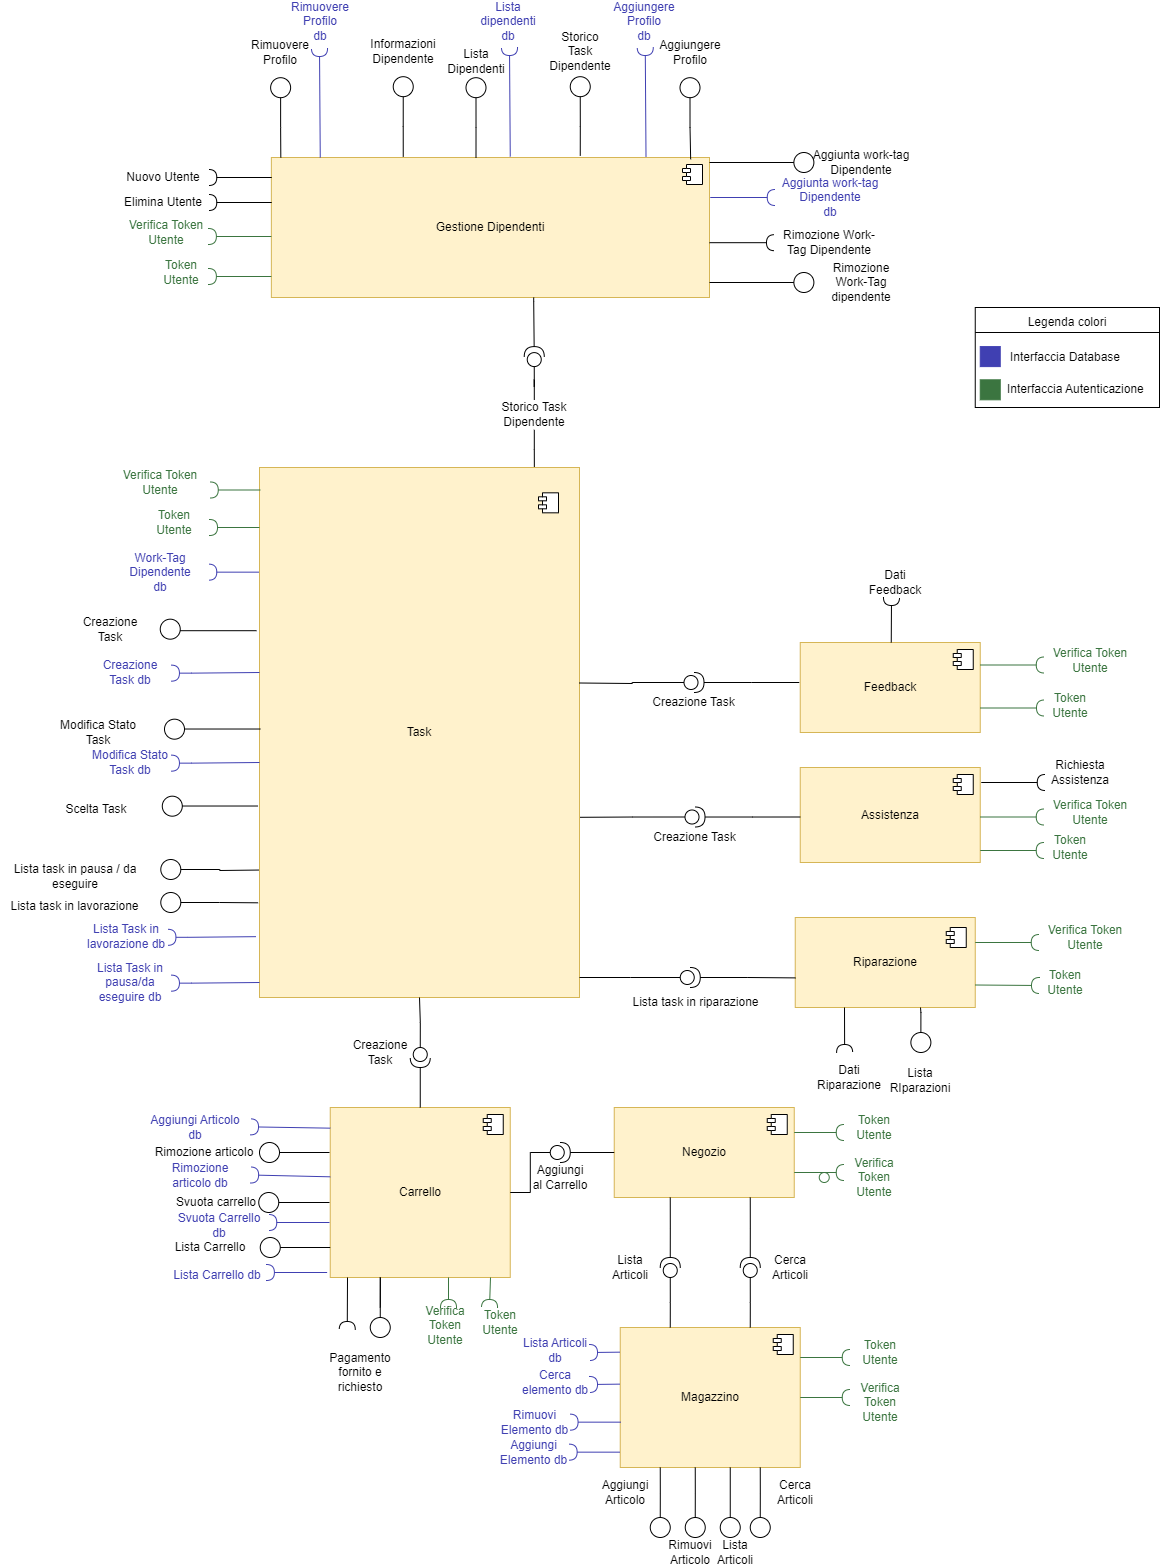
\includegraphics[width=1\textwidth]{images/diagramma_dei_componenti.png}
	Diagramma delle Componenti 2 per l'applicazione FixMi
\end{figure}
A seguire una descrizione dei componenti e delle interfacce presenti nel diagramma.

\subsection*{Autenticazione}
\textbf{Descrizione}: Questa componente si occupa del controllo dell'accesso ai servizi dell'applicazione da parte degli utenti,
e fornisce un metodo di verifica dei dati di autenticazione degli utenti alle altre componenti che li richiedono.
\subsubsection*{\indent  \indent Sistema Token}
\uline{\textit{Interfaccia fornita - Token utente}}: 
La componente fornisce il token di un determinato utente alle componenti che lo richiedono.\\ \\ 
\uline{\textit{Interfaccia fornita - Verifica token utente}}: 
La componente verifica l'esistenza di un determinato utente su richiesta di altre componenti, comunicando anche il ruolo di quel determinato utente.

\subsubsection*{\indent \indent Verifica dati Autenticazione}
\uline{\textit{Interfaccia richiesta - Dati autenticazione utente db}}: 
La componente richiede al database i dati personali di un determinato utente data l'email dello stesso. Questi dati sono:
\begin{itemize}
	\item username
	\item password hash
	\item ruolo (cliente, dipendente o manager)
\end{itemize}
\uline{\textit{Interfaccia fornita - Verifica credenziali}}: 
La componente, su richiesta di altre componenti, verifica che le credenziali(Email e password) di un determinato utente siano corrette.\\ \\ 
\uline{\textit{Interfaccia fornita - Verifica esistenza email}}: 
La componente verifica se la mail fornita è già registrata in un account utente.

\subsubsection*{ \indent  \indent Creazione, modifica ed eliminazione utenti}
\uline{\textit{Interfaccia fornita - Nuovo utente}}: 
La componente riceve i dati per la creazione di un nuovo utente. I dati sono i seguenti:
\begin{itemize}
	\item username
	\item email
	\item password
	\item ruolo (cliente dipendente o manager)
\end{itemize}
\uline{\textit{Interfaccia richiesta - Nuovo utente db}}: 
La componente fornisce al database i seguenti dati per la creazione di un nuovo utente.
\begin{itemize}
	\item username
	\item email
	\item password hash
	\item ruolo (cliente, dipendente o manager)
	
\end{itemize}
\uline{\textit{Interfaccia fornita - Aggiorna password}}:
La componente, su richiesta di altre componenti, aggiorna la password di un determinato utente.\\\\
\uline{\textit{Interfaccia richiesta - Aggiorna password db}}: 
La componente aggiorna la hash della password di un determinato utente sul database.  \\\\
\uline{\textit{Interfaccia Richiesta - Elimina utente db}}: 
La componente richiede al database l'eliminazione dei dati di un determinato utente.\\\\
\uline{\textit{Interfaccia Fornita - Elimina utente}}: 
La componente fornisce alle altre componenti la possibilità di eliminare i dati di un determinato utente.

\subsection*{Login}
\textbf{Descrizione}: Questa componente si occupa del processo di login, descritto in RF1.
\subsubsection*{\indent \indent Credenziali}
\uline{\textit{Interfaccia richiesta - Email e password}}: 
Viene richiesta l'email e la password all'ospite che vuole autenticarsi.\\ \\ 
\uline{\textit{Interfaccia richiesta - Verifica credenziali}}: 
La componente richiede la verifica delle credenziali(E-mail e password) dell'ospite che vuole autenticarsi alla componente Autenticazione.
\subsubsection*{\indent \indent 2 Factor Authentication}
\uline{\textit{Interfaccia richiesta - Invio Codice 2FA}}: 
La componente fornisce al E-mail Server il codice 2 Factor Authentication da inviare alla E-mail dell'utente.\\ \\
\uline{\textit{Interfaccia richiesta - Controllo 2FA}}: 
Viene richiesto all'utente l'inserimento del codice 2 Factor Authentication ricevuto tramite mail. 
\subsubsection*{\indent \indent Sistema Token}
\uline{\textit{Interfaccia richiesta - Token utente}}: 
Viene richiesto alla componente "Autenticazione" il token dell'utente appena autenticato, per poi inviarlo all'utente.

\subsection*{Cambio password}
\textbf{Descrizione}: Questa componente si occupa del processo di cambio password, descritto in RF1.\\ \\ 

\uline{\textit{Interfaccia richiesta - E-mail}}: 
Viene richiesta la propria E-Mail all'utente che vuole cambiare password .\\ \\
\uline{\textit{Interfaccia richiesta - Verifica esistenza email}}: 
La componente richiede alla componente "Autenticazione" l'esistenza di un profilo utente con la email fornita. 
\subsubsection*{\indent \indent 2 Factor Authentication}
\uline{\textit{Interfaccia richiesta - Invio Codice 2FA}}: 
La componente fornisce al Email Server il codice 2 Factor Authentication da inviare all'utente.\\ \\ 
\uline{\textit{Interfaccia richiesta - Controllo 2FA}}:
Viene richiesto all'utente l'inserimento del codice 2 Factor Authentication appena ricevuto.
\subsubsection*{\indent \indent Aggiornamento Password}
\uline{\textit{Interfaccia richiesta - Nuova password}}: 
Viene richiesto all'utente l'inserimento della nuova password.\\ \\
\uline{\textit{Interfaccia richiesta - Aggiorna password}}: 
La componente richiede alla componente autenticazione l'aggiornamento della password precedente dell'account utente con quella appena inserita.

\subsection*{Registrazione}
\textbf{Descrizione}: Questa componente si occupa del processo di registrazione, descritto in RF2.
\subsubsection*{\indent \indent Credenziali}
\uline{\textit{Interfaccia richiesta - Dati registrazione utente}}: 
Per registrarsi, vengono richiesti all'ospite i seguenti dati:
\begin{itemize}
	\item email
	\item password
	\item conferma password
	\item username
\end{itemize}
\uline{\textit{Interfaccia richiesta - Verifica esistenza email}}: 
La componente richiede alla componente "Autenticazione" l'esistenza di un utente con la mail fornita,
per decidere se procedere o meno con la registrazione.
\subsubsection*{\indent \indent 2 Factor Authentication}
\uline{\textit{Interfaccia richiesta - Invio Codice 2FA}}: 
La componente fornisce il codice 2 Factor Authentication al Email Server, da inviare all'ospite che vuole registrarsi.\\ \\ 
\uline{\textit{Interfaccia richiesta - Controllo 2FA}}: 
La componente richiede all'ospite il codice 2FA appena ricevuto tramite e-mail.
\subsubsection*{\indent \indent Creazione Utente}
\uline{\textit{Interfaccia richiesta - Nuovo utente}}: 
Vengono forniti i dati della registrazione dell'utente al componente "Autenticazione", con il ruolo "cliente".\\ \\ 
\uline{\textit{Interfaccia richiesta - Token utente}}: 
Viene richiesto alla componente "Autenticazione" il token dell'utente appena registrato.
\subsubsection*{\indent \indent Sistema Token}
\uline{\textit{Interfaccia fornita - Token utente}}: 
Viene fornito all'utente il proprio token.

\iffalse
\subsection*{Server mail}
\textbf{Descrizione}: Questa componente si occupa dell'invio delle e-mail 2FA \\ \\
\uline{\textit{Interfaccia fornita - Invio Codice 2FA}}:
La componente fornisce la possibilità di inviare una mail con un codice 2FA all'email di un determinato utente.
\fi
\subsection*{Negozio}
\textbf{Descrizione}: Questa componente si occupa di mostrare  ed interagire con il negozio ad ogni tipo di utente in base al livello di privilegi dello stesso. In particolare permette di ricercare un articolo nel negozio, ordinarlo in ordine alfabetico e permettere di aggiungere un prodotto al carrello.\\\\
\uline{\textit{Interfaccia Richiesta - Lista Articoli}}: 
Il Negozio si aspetta di ricevere la lista degli articoli presenti nel magazzino per poterli mostrare, ossia il nome dell'articolo, una foto e una descrizione. \\ \\
\uline{\textit{Interfaccia Richiesta - Cerca Articoli}}: 
Il Negozio può visualizzare la lista degli articoli presenti nel magazzino tali che il nome contiene una stringa di ricerca.\\\\
\uline{\textit{Interfaccia Richiesta - Aggiungi al Carrello}}: 
Tramite il negozio si può aggiungere un elemento al carrello prima di poterlo acquistare. 
\subsubsection*{\indent \indent Identificazione Utente}
\uline{\textit{Interfaccia Richiesta - Token Utente}}: 
Viene richiesto all'utente il proprio token identificativo.\\ \\
\uline{\textit{Interfaccia Richiesta - Verifica Token Utente}}: 
La componente richiede la verifica del token utente alla componente "Autenticazione".\\\\

\subsection*{Carrello}
\textbf{Descrizione}: Questa componente registra l'inserimento e la rimozione degli articoli nel carrello e permette di effettuare l'acquisto di tali articoli. 
\subsubsection*{\indent \indent Identificazione Utente}
\uline{\textit{Interfaccia Richiesta - Token Utente}}: 
Viene richiesto all'utente il proprio token identificativo\\ \\
\uline{\textit{Interfaccia Richiesta - Verifica Token Utente}}: 
La componente richiede la verifica del token utente alla componente "Autenticazione"
\subsubsection*{\indent \indent Lettura}
\uline{\textit{Interfaccia Richiesta - Lista carrello db}}: 
La componente richiede al database gli elementi del carrello di un determinato utente. \\\\
\uline{\textit{Interfaccia Fornita - Lista carrello}}: 
La componente fornisce il proprio carrello all'utente che lo richiede.
\subsubsection*{\indent \indent Inserimento}
\uline{\textit{Interfaccia Richiesta - Aggiungi Articolo db}}:
 La componente richiede al database di salvare un articolo nel carrello di un determinato utente\\\\ 
\uline{\textit{Interfaccia Fornita - Aggiungi al Carrello}}: 
Il carrello permette al Negozio di poter aggiungere articoli e salvarli nel carrello.
%\uline{\textit{Interfaccia Richiesta - Aggiungi Articolo}}: Il Carrello si interfaccia con un database per il salvataggio degli articoli nel carrello oltre la sessione.\\ \\
\subsubsection*{\indent \indent Eliminazione}
\uline{\textit{Interfaccia Richiesta - Rimozione Articolo db}}: 
Il Carrello si interfaccia con un database per rimuovere un articolo dal carrello in modo permanente.\\ \\
\uline{\textit{Interfaccia Fornita - Rimozione Articolo}}: 
Il Carrello fornisce all'utente la possibilità di rimuovere elementi dal carrello\\\\
\uline{\textit{Interfaccia Richiesta - Svuota Carrello db}}: 
Il Carrello si interfaccia con un database per svuotare tutti i dati degli articoli presenti nel carrello in modo permanente.\\ \\
\uline{\textit{Interfaccia Fornita - Svuota Carrello}}:
Il Carrello fornisce all'utente la possibilità di rimuovere tutti gli articoli dal proprio carrello
\subsubsection*{\indent \indent Pagamento}
\uline{\textit{Interfaccia Richiesta - Pagamento}}:
Il Carrello si interfaccia con un sistema esterno per effettuare il pagamento degli articoli salvati nel carrello.\\\\
\uline{\textit{Interfaccia Fornita - Pagamento}}:
Il carrello fornisce all'utente la possibilità di pagare utilizzando Nexi o Paypal.
\subsubsection*{\indent \indent Sistema Task}
\uline{\textit{Interfaccia Richiesta - Creazione Task}}:
La componente richiede alla componente "Task" la creazione di una task "Magazzino", specificando i prodotti acquistati dall'utente.
% Non so se assistenza, feedback e riparazione vanno qua dentro
\subsection*{Riparazione}
\textbf{Descrizione}: Questa componente si occupa di prendere le richieste di riparazione degli utenti e di mostrare quelle già richieste.
\subsubsection*{\indent \indent Identificazione Utente}
\uline{\textit{Interfaccia Richiesta - Token utente}}: 
Viene richiesto all'utente il proprio token identificativo.\\\\
\uline{\textit{Interfaccia Richiesta - Verifica token utente}}:
La componente richiede la verifica del token utente alla componente "Autenticazione".
\subsubsection*{\indent \indent Richiesta Riparazione}
\uline{\textit{Interfaccia Richiesta - Dati riparazione}}:
La componente richiede all'utente le informazioni riguardanti la richiesta di riparazione:
\begin{itemize}
	\item telefono
	\item email
	\item cognome
	\item nome
	\item descrizione
	\item foto(opzionale)
\end{itemize}
\uline{\textit{Interfaccia richiesta - Creazione task}}: 
La componente richiede alla componente "Task" la creazione di una nuova task riparazione con i dettagli inseriti dall'utente.
\subsubsection*{\indent \indent Lista}
\uline{\textit{Interfaccia fornita - Lista riparazioni}}: %questa la lasciamo come interfaccia??
La componente fornisce all'utente la lista delle riparazioni che ha richiesto in precedenza.\\\\
\uline{\textit{Interfaccia richiesta - Lista task riparazione}}: 
La componente richiede alla componente "Task" la lista delle riparazioni richieste dall'utente in precedenza.

\subsection*{Assistenza}
\textbf{Descrizione}: Questa componente si occupa di raccogliere le richieste di assistenza degli utenti.
\subsubsection*{\indent \indent Identificazione Utente}
\uline{\textit{Interfaccia Richiesta - Token utente}}: 
Viene richiesto all'utente il proprio token identificativo.\\\\
\uline{\textit{Interfaccia Richiesta - Verifica token utente}}:
La componente richiede la verifica del token utente alla componente "Autenticazione".
\subsubsection*{\indent \indent Richiesta Assistenza}
\uline{\textit{Interfaccia Richiesta - Richiesta assistenza}}:
La componente richiede all'utente le informazioni riguardanti la propria richiesta di assistenza:
\begin{itemize}
	\item descrizione
	\item e-mail
\end{itemize}
\uline{\textit{Interfaccia Richiesta - Creazione task}}:
La componente richiede alla componente "Task" la creazione di una nuova task "assistenza" con i dettagli inseriti dall'utente.

\subsection*{Feedback}
\textbf{Descrizione}: Questa componente si occupa di raccogliere i feedback degli utenti.
\subsubsection*{\indent \indent Identificazione Utente}
\uline{\textit{Interfaccia Richiesta - Token utente}}: 
Viene richiesto all'utente il proprio token identificativo\\ \\
\uline{\textit{Interfaccia Richiesta - Verifica token utente}}:
La componente richiede la verifica del token utente alla componente "Autenticazione".
\subsubsection*{\indent \indent Invio Feedback}
\uline{\textit{Interfaccia Richiesta - Dati feedback}}:
La componente richiede all'utente le informazioni riguardanti il feedback che desidera inviare:
\begin{itemize}
	\item disponibilità azienda
	\item velocità riparazione
	\item soddisfazione riparazione
	\item soddisfazione sito web
	\item idee per migliorare
\end{itemize}
\uline{\textit{Interfaccia Richiesta - Creazione Task}}:
La componente richiede alla componente "Task" la creazione di una nuova task "assistenza" con i dettagli inseriti dall'utente.

\subsection*{Magazzino}
\textbf{Descrizione: } Questa componente permette il salvataggio e rimozione degli articoli in un database esterno.
\subsubsection*{ \indent \indent Identificazione Utente}
\uline{\textit{Interfaccia Richiesta - Token Utente}}:
Viene richiesto all'utente il proprio token identificativo.\\ \\
\uline{\textit{Interfaccia Richiesta - Verifica Token Utente}}: 
La componente richiede la verifica del token utente alla componente "Autenticazione", anche per verificare che abbia il ruolo adeguato.
\subsubsection*{\indent \indent Inserimento}
\uline{\textit{Interfaccia Fornita - Aggiungi Articolo}}:
Il Magazzino permette all'utente di aggiungere un articolo al magazzino  \\ \\%specificando cosa?
\uline{\textit{Interfaccia Richiesta - Aggiungi Elemento db}}:
Il Magazzino si interfaccia con un database esterno per il salvataggio degli articoli.
\subsubsection*{\indent \indent Lettura}
\uline{\textit{Interfaccia Fornita - Lista Articoli}}:
Il Magazzino permette ad altre componenti di aver accesso a tutti articoli presenti, inoltre la lista può essere inviata in senso alfabetico crescente o descrescente.\\ \\
\uline{\textit{interfaccia Fornita - Cerca Articoli}}:
Il Magazzino permette di ricercare gli articoli la cui descrizione contiene una certa stringa.\\ \\
\uline{\textit{Interfaccia Richiesta - Lista Articoli db}}:
Il Magazzino si interfaccia con un database esterno per ottenere una lista degli articoli salvati del database.\\ \\
\uline{\textit{Interfaccia Richiesta - Cerca elemento db}}:
Il Magazzino si interfaccia con un database esterno per cercare gli articoli che contengono una stringa nel nome.
\subsubsection*{\indent \indent Eliminazione}
\uline{\textit{Interfaccia Fornita - Rimuovi Articolo}}:
Il Magazzino permette la rimozione di un articolo dallo stesso.\\ \\
\uline{\textit{Interfaccia Richiesta - Rimuovi Elemento db}}:
Il Magazzino si interfaccia con un database esterno per la rimozione permanente di un articolo.
\subsection*{Task}

\textbf{Descrizione}: Questa componente si occupa di gestire il sistema task della applicazione.
\subsubsection*{\indent \indent Identificazione Utente}
\uline{\textit{Interfaccia Richiesta - Token Utente}}:
La componente richiede al dipendente(o manager) il proprio token utente \\ \\
\uline{\textit{Interfaccia Richiesta - Verifica token utente}}: 
La componente richiede la verifica del token utente alla componente "Autenticazione", per verificare se ha il ruolo adeguato per poter accedere. \\ \\ 
\uline{\textit{Interfaccia Richiesta - work-tag dipendente db}}: 
La componente richiede al database le work-tag di un determinato dipendente. 
\subsubsection*{\indent \indent Creazione}
\uline{\textit{Interfaccia Fornita - Creazione task}}: 
La componente fornisce la possibilità di creare una task da parte delle componenti che lo richiedono. \\\\
\uline{\textit{Interfaccia Richiesta - Creazione task db}}:
La componente richiede al database di creare una task. 
\subsubsection*{\indent \indent Lettura}
\uline{\textit{Interfaccia richiesta - Lista task in lavorazione db}}: 
La componente richiede al database la lista delle task in lavorazione, filtrata in base a vari filtri.\\\\
\uline{\textit{Interfaccia fornita - Lista task in lavorazione}}: 
La componente permette al dipendente di vedere  la lista delle task in lavorazione.\\\\
\uline{\textit{Interfaccia richiesta - Lista task in pausa/da eseguire db}}: 
La componente richiede al database la lista delle task in pausa/da eseguire, filtrata in base a vari filtri.\\\\
\uline{\textit{Interfaccia fornita - Lista task in pausa/da eseguire}}: 
La componente permette al dipendente di vedere la lista delle task che può eseguire.\\\\
\uline{\textit{Interfaccia fornita - Lista task riparazione}}:
La componente permette alla componente "Riparazione" di richiedere la lista delle riparazioni richieste da un determinato cliente.\\\\
\uline{\textit{Interfaccia fornita - Storico task dipendente}}:
La componente permette alla componente "Gestione Dipendenti" di richiedere la lista delle task svolte/in svolgimento di un determinato dipendente.
\subsubsection*{\indent \indent Modifica}
\uline{\textit{Interfaccia fornita - Scelta task}}: 
La componente permette al dipendente di scegliere una task da eseguire.\\\\
\uline{\textit{Interfaccia richiesta - modifica stato task db}}:
 La componente richiede al database di modificare lo stato di una task.\\\\
\uline{\textit{Interfaccia fornita - modifica stato task}}: 
La componente permette al dipendente di modificare lo stato della task scelta.



\subsection*{Gestione Dipendenti}
\textbf{Descrizione}: Questa componente si occupa della gestione dei profili dei dipendenti, della loro creazione,modifica e eliminazione.
\subsubsection*{\indent \indent Identificazione Utente}
\uline{\textit{Interfaccia Richiesta - Token Utente}}:
La componente richiede al manager il proprio token utente. \\ \\
\uline{\textit{Interfaccia Richiesta - Verifica token utente}}: 
La componente richiede la verifica del token utente alla componente "Autenticazione", per verificare se ha il ruolo adeguato per poter accedere.
\subsubsection*{\indent \indent Lettura}
\uline{\textit{Interfaccia Richiesta - Lista dipendenti db}}:
La componente richiede al database la lista dei dipendenti e le corrispettive informazioni anagrafiche.\\\\
\uline{\textit{Interfaccia Fornita - Lista dipendenti}}:
La componente fornisce al manager la lista dei dipendenti.\\\\
\uline{\textit{Interfaccia Fornita - Informazioni dipendente}}:
La componente fornisce al manager le informazioni di un determinato dipendente.
\subsubsection*{\indent \indent Eliminazione}
\uline{\textit{Interfaccia Fornita - Rimuovere profilo}}:
La componente fornisce al manager la possibilità di rimuovere un profilo dipendente.\\\\
\uline{\textit{Interfaccia Richiesta - Rimuovere profilo db}}:
La componente richiede al database la rimozione di un profilo dipendente dal database.\\\\
\uline{\textit{Interfaccia Richiesta - Elimina utente}}:
La componente richiede alla componente "Autenticazione" l'eliminazione dei dati di autenticazione associati a un determinato dipendente. 
\subsubsection*{\indent \indent Inserimento}
\uline{\textit{Interfaccia Fornita - Aggiungere profilo}}:
La componente fornisce al manager la possibilità di aggiungere un nuovo profilo dipendente inserendo i seguenti parametri:
\begin{itemize}
	\item nome dipendente
	\item cognome dipendente
	\item data di nascita
	\item data di assunzione
	\item email 
	\item password
	\item foto(opzionale)
\end{itemize}
\uline{\textit{Interfaccia Richiesta - Nuovo utente}}: 
La componente richiede alla componente "Autenticazione" la creazione di un nuovo utente con i seguenti campi
\begin{itemize}
	\item username: nome del dipendente fornito dal manager
	\item email: email del dipendente fornita dal manager
	\item password: password del dipendente fornita dal manager
\end{itemize}
\uline{\textit{Interfaccia Richiesta - Aggiungere profilo db}}:
La componente richiede al database l'aggiunta di un nuovo profilo dipendente con i seguenti campi:
\begin{itemize}
	\item nome dipendente
	\item cognome dipendente
	\item data di nascita
	\item data di assunzione
	\item foto(opzionale)
\end{itemize}.
\subsubsection*{\indent \indent Work-Tag Dipendente}
\uline{\textit{Interfaccia Richiesta -Aggiunta work-tag dipendente db}}:
La componente richiede al database l'aggiunta di una work-tag al profilo di un determinato dipendente.\\\\
\uline{\textit{Interfaccia Fornita - Aggiunta work-tag dipendente}}:
La componente fornisce al manager la possibilità di aggiungere una work-tag a un determinato dipendente.\\\\
\uline{\textit{Interfaccia Richiesta - Rimozione work-tag dipendente db}}:
La componente richiede al database l'aggiunta di una work-tag al profilo di un determinato dipendente.\\\\
\uline{\textit{Interfaccia Fornita - Rimozione work-tag dipendente}}:
La componente fornisce al manager la possibilità di eliminare una work-tag di un determinato dipendente.
\subsubsection*{\indent \indent Storico Task Dipendente}
\uline{\textit{Interfaccia richiesta - Storico task dipendente}}:
La componente richiede alla componente "Task" lo storico delle task di un determinato dipendente.\\\\
\uline{\textit{Interfaccia fornita - Storico task dipendente}}:
La componente fornisce al manager la possibilità di visualizzare lo storico delle task di un determinato dipendente.

\end{document}